\subsection{The DNA Section}

\begin{figure}
\centering
% Created by tikzDevice version 0.12.3.1 on 2022-10-19 12:01:19
% !TEX encoding = UTF-8 Unicode
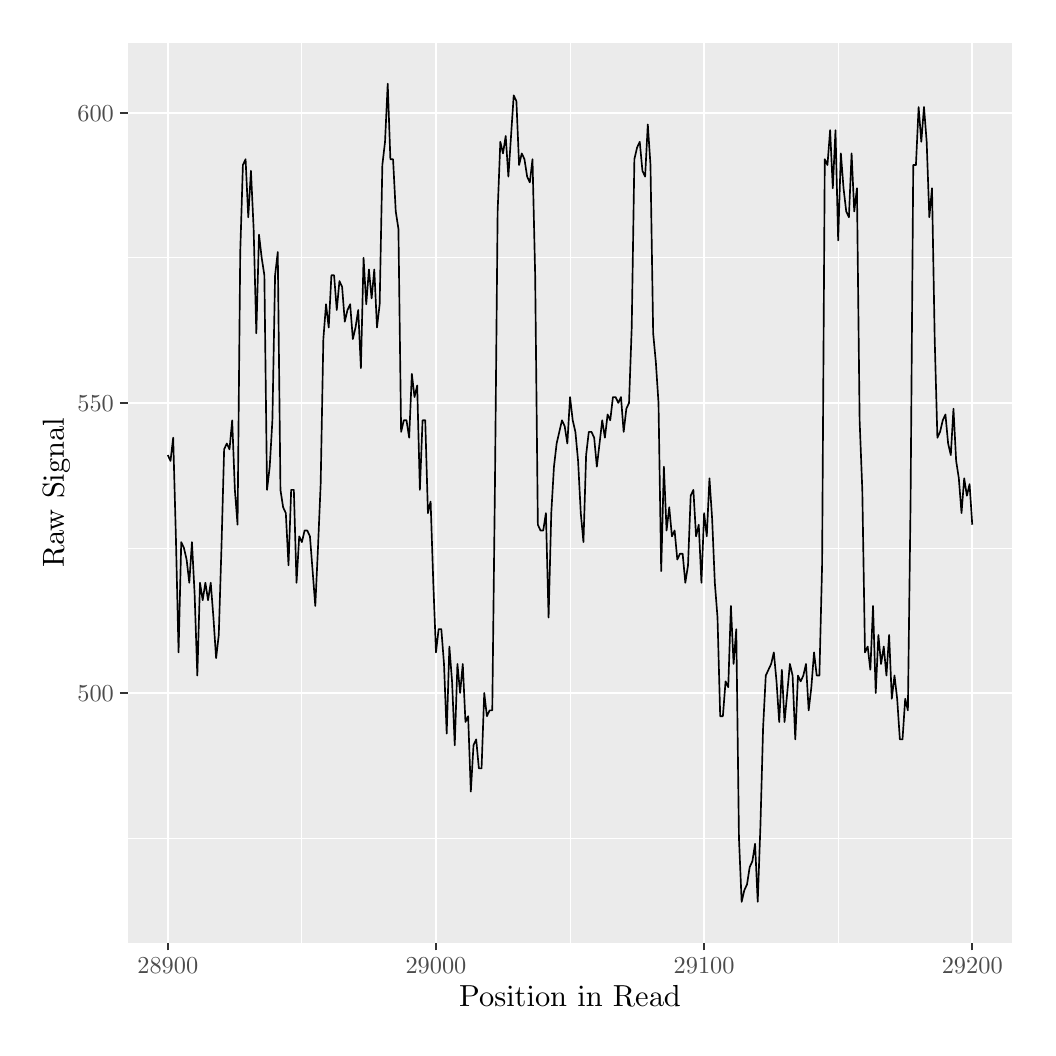
\begin{tikzpicture}[x=1pt,y=1pt]
\definecolor{fillColor}{RGB}{255,255,255}
\path[use as bounding box,fill=fillColor,fill opacity=0.00] (0,0) rectangle (361.35,361.35);
\begin{scope}
\path[clip] (  0.00,  0.00) rectangle (361.35,361.35);
\definecolor{drawColor}{RGB}{255,255,255}
\definecolor{fillColor}{RGB}{255,255,255}

\path[draw=drawColor,line width= 0.6pt,line join=round,line cap=round,fill=fillColor] (  0.00,  0.00) rectangle (361.35,361.35);
\end{scope}
\begin{scope}
\path[clip] ( 36.11, 30.69) rectangle (355.85,355.85);
\definecolor{fillColor}{gray}{0.92}

\path[fill=fillColor] ( 36.11, 30.69) rectangle (355.85,355.85);
\definecolor{drawColor}{RGB}{255,255,255}

\path[draw=drawColor,line width= 0.3pt,line join=round] ( 36.11, 68.53) --
	(355.85, 68.53);

\path[draw=drawColor,line width= 0.3pt,line join=round] ( 36.11,173.35) --
	(355.85,173.35);

\path[draw=drawColor,line width= 0.3pt,line join=round] ( 36.11,278.18) --
	(355.85,278.18);

\path[draw=drawColor,line width= 0.3pt,line join=round] ( 99.09, 30.69) --
	( 99.09,355.85);

\path[draw=drawColor,line width= 0.3pt,line join=round] (195.98, 30.69) --
	(195.98,355.85);

\path[draw=drawColor,line width= 0.3pt,line join=round] (292.87, 30.69) --
	(292.87,355.85);

\path[draw=drawColor,line width= 0.6pt,line join=round] ( 36.11,120.94) --
	(355.85,120.94);

\path[draw=drawColor,line width= 0.6pt,line join=round] ( 36.11,225.76) --
	(355.85,225.76);

\path[draw=drawColor,line width= 0.6pt,line join=round] ( 36.11,330.59) --
	(355.85,330.59);

\path[draw=drawColor,line width= 0.6pt,line join=round] ( 50.64, 30.69) --
	( 50.64,355.85);

\path[draw=drawColor,line width= 0.6pt,line join=round] (147.54, 30.69) --
	(147.54,355.85);

\path[draw=drawColor,line width= 0.6pt,line join=round] (244.43, 30.69) --
	(244.43,355.85);

\path[draw=drawColor,line width= 0.6pt,line join=round] (341.32, 30.69) --
	(341.32,355.85);
\definecolor{drawColor}{RGB}{0,0,0}

\path[draw=drawColor,line width= 0.6pt,line join=round] ( 50.64,206.90) --
	( 51.61,204.80) --
	( 52.58,213.18) --
	( 53.55,177.54) --
	( 54.52,135.61) --
	( 55.49,175.45) --
	( 56.46,173.35) --
	( 57.43,169.16) --
	( 58.40,160.77) --
	( 59.36,175.45) --
	( 60.33,156.58) --
	( 61.30,127.23) --
	( 62.27,160.77) --
	( 63.24,154.48) --
	( 64.21,160.77) --
	( 65.18,154.48) --
	( 66.15,160.77) --
	( 67.12,148.19) --
	( 68.09,133.52) --
	( 69.05,141.90) --
	( 70.02,173.35) --
	( 70.99,208.99) --
	( 71.96,211.09) --
	( 72.93,208.99) --
	( 73.90,219.47) --
	( 74.87,194.32) --
	( 75.84,181.74) --
	( 76.81,280.27) --
	( 77.77,311.72) --
	( 78.74,313.82) --
	( 79.71,292.85) --
	( 80.68,309.62) --
	( 81.65,288.66) --
	( 82.62,250.92) --
	( 83.59,286.56) --
	( 84.56,278.18) --
	( 85.53,271.89) --
	( 86.49,194.32) --
	( 87.46,202.70) --
	( 88.43,219.47) --
	( 89.40,271.89) --
	( 90.37,280.27) --
	( 91.34,194.32) --
	( 92.31,188.03) --
	( 93.28,185.93) --
	( 94.25,167.06) --
	( 95.21,194.32) --
	( 96.18,194.32) --
	( 97.15,160.77) --
	( 98.12,177.54) --
	( 99.09,175.45) --
	(100.06,179.64) --
	(101.03,179.64) --
	(102.00,177.54) --
	(102.97,164.97) --
	(103.93,152.39) --
	(104.90,173.35) --
	(105.87,196.41) --
	(106.84,248.82) --
	(107.81,261.40) --
	(108.78,253.02) --
	(109.75,271.89) --
	(110.72,271.89) --
	(111.69,259.31) --
	(112.65,269.79) --
	(113.62,267.69) --
	(114.59,255.11) --
	(115.56,259.31) --
	(116.53,261.40) --
	(117.50,248.82) --
	(118.47,253.02) --
	(119.44,259.31) --
	(120.41,238.34) --
	(121.37,278.18) --
	(122.34,261.40) --
	(123.31,273.98) --
	(124.28,263.50) --
	(125.25,273.98) --
	(126.22,253.02) --
	(127.19,261.40) --
	(128.16,311.72) --
	(129.13,320.11) --
	(130.10,341.07) --
	(131.06,313.82) --
	(132.03,313.82) --
	(133.00,294.95) --
	(133.97,288.66) --
	(134.94,215.28) --
	(135.91,219.47) --
	(136.88,219.47) --
	(137.85,213.18) --
	(138.82,236.25) --
	(139.78,227.86) --
	(140.75,232.05) --
	(141.72,194.32) --
	(142.69,219.47) --
	(143.66,219.47) --
	(144.63,185.93) --
	(145.60,190.12) --
	(146.57,160.77) --
	(147.54,135.61) --
	(148.50,144.00) --
	(149.47,144.00) --
	(150.44,131.42) --
	(151.41,106.26) --
	(152.38,137.71) --
	(153.35,125.13) --
	(154.32,102.07) --
	(155.29,131.42) --
	(156.26,120.94) --
	(157.22,131.42) --
	(158.19,110.46) --
	(159.16,112.55) --
	(160.13, 85.30) --
	(161.10,102.07) --
	(162.07,104.17) --
	(163.04, 93.69) --
	(164.01, 93.69) --
	(164.98,120.94) --
	(165.94,112.55) --
	(166.91,114.65) --
	(167.88,114.65) --
	(168.85,196.41) --
	(169.82,294.95) --
	(170.79,320.11) --
	(171.76,315.91) --
	(172.73,322.20) --
	(173.70,307.53) --
	(174.66,322.20) --
	(175.63,336.88) --
	(176.60,334.78) --
	(177.57,311.72) --
	(178.54,315.91) --
	(179.51,313.82) --
	(180.48,307.53) --
	(181.45,305.43) --
	(182.42,313.82) --
	(183.38,271.89) --
	(184.35,181.74) --
	(185.32,179.64) --
	(186.29,179.64) --
	(187.26,185.93) --
	(188.23,148.19) --
	(189.20,185.93) --
	(190.17,202.70) --
	(191.14,211.09) --
	(192.10,215.28) --
	(193.07,219.47) --
	(194.04,217.38) --
	(195.01,211.09) --
	(195.98,227.86) --
	(196.95,219.47) --
	(197.92,215.28) --
	(198.89,204.80) --
	(199.86,185.93) --
	(200.83,175.45) --
	(201.79,206.90) --
	(202.76,215.28) --
	(203.73,215.28) --
	(204.70,213.18) --
	(205.67,202.70) --
	(206.64,211.09) --
	(207.61,219.47) --
	(208.58,213.18) --
	(209.55,221.57) --
	(210.51,219.47) --
	(211.48,227.86) --
	(212.45,227.86) --
	(213.42,225.76) --
	(214.39,227.86) --
	(215.36,215.28) --
	(216.33,223.67) --
	(217.30,225.76) --
	(218.27,253.02) --
	(219.23,313.82) --
	(220.20,318.01) --
	(221.17,320.11) --
	(222.14,309.62) --
	(223.11,307.53) --
	(224.08,326.39) --
	(225.05,311.72) --
	(226.02,250.92) --
	(226.99,240.44) --
	(227.95,225.76) --
	(228.92,164.97) --
	(229.89,202.70) --
	(230.86,179.64) --
	(231.83,188.03) --
	(232.80,177.54) --
	(233.77,179.64) --
	(234.74,169.16) --
	(235.71,171.25) --
	(236.67,171.25) --
	(237.64,160.77) --
	(238.61,167.06) --
	(239.58,192.22) --
	(240.55,194.32) --
	(241.52,177.54) --
	(242.49,181.74) --
	(243.46,160.77) --
	(244.43,185.93) --
	(245.39,177.54) --
	(246.36,198.51) --
	(247.33,183.83) --
	(248.30,160.77) --
	(249.27,148.19) --
	(250.24,112.55) --
	(251.21,112.55) --
	(252.18,125.13) --
	(253.15,123.04) --
	(254.11,152.39) --
	(255.08,131.42) --
	(256.05,144.00) --
	(257.02, 68.53) --
	(257.99, 45.47) --
	(258.96, 49.66) --
	(259.93, 51.76) --
	(260.90, 58.04) --
	(261.87, 60.14) --
	(262.84, 66.43) --
	(263.80, 45.47) --
	(264.77, 72.72) --
	(265.74,108.36) --
	(266.71,127.23) --
	(267.68,129.33) --
	(268.65,131.42) --
	(269.62,135.61) --
	(270.59,125.13) --
	(271.56,110.46) --
	(272.52,129.33) --
	(273.49,110.46) --
	(274.46,120.94) --
	(275.43,131.42) --
	(276.40,127.23) --
	(277.37,104.17) --
	(278.34,127.23) --
	(279.31,125.13) --
	(280.28,127.23) --
	(281.24,131.42) --
	(282.21,114.65) --
	(283.18,123.04) --
	(284.15,135.61) --
	(285.12,127.23) --
	(286.09,127.23) --
	(287.06,167.06) --
	(288.03,313.82) --
	(289.00,311.72) --
	(289.96,324.30) --
	(290.93,303.33) --
	(291.90,324.30) --
	(292.87,284.46) --
	(293.84,315.91) --
	(294.81,303.33) --
	(295.78,294.95) --
	(296.75,292.85) --
	(297.72,315.91) --
	(298.68,294.95) --
	(299.65,303.33) --
	(300.62,219.47) --
	(301.59,194.32) --
	(302.56,135.61) --
	(303.53,137.71) --
	(304.50,129.33) --
	(305.47,152.39) --
	(306.44,120.94) --
	(307.40,141.90) --
	(308.37,131.42) --
	(309.34,137.71) --
	(310.31,127.23) --
	(311.28,141.90) --
	(312.25,118.84) --
	(313.22,127.23) --
	(314.19,118.84) --
	(315.16,104.17) --
	(316.12,104.17) --
	(317.09,118.84) --
	(318.06,114.65) --
	(319.03,190.12) --
	(320.00,311.72) --
	(320.97,311.72) --
	(321.94,332.68) --
	(322.91,320.11) --
	(323.88,332.68) --
	(324.85,320.11) --
	(325.81,292.85) --
	(326.78,303.33) --
	(327.75,248.82) --
	(328.72,213.18) --
	(329.69,215.28) --
	(330.66,219.47) --
	(331.63,221.57) --
	(332.60,211.09) --
	(333.57,206.90) --
	(334.53,223.67) --
	(335.50,204.80) --
	(336.47,198.51) --
	(337.44,185.93) --
	(338.41,198.51) --
	(339.38,192.22) --
	(340.35,196.41) --
	(341.32,181.74);
\end{scope}
\begin{scope}
\path[clip] (  0.00,  0.00) rectangle (361.35,361.35);
\definecolor{drawColor}{gray}{0.30}

\node[text=drawColor,anchor=base east,inner sep=0pt, outer sep=0pt, scale=  0.88] at ( 31.16,117.91) {500};

\node[text=drawColor,anchor=base east,inner sep=0pt, outer sep=0pt, scale=  0.88] at ( 31.16,222.73) {550};

\node[text=drawColor,anchor=base east,inner sep=0pt, outer sep=0pt, scale=  0.88] at ( 31.16,327.56) {600};
\end{scope}
\begin{scope}
\path[clip] (  0.00,  0.00) rectangle (361.35,361.35);
\definecolor{drawColor}{gray}{0.20}

\path[draw=drawColor,line width= 0.6pt,line join=round] ( 33.36,120.94) --
	( 36.11,120.94);

\path[draw=drawColor,line width= 0.6pt,line join=round] ( 33.36,225.76) --
	( 36.11,225.76);

\path[draw=drawColor,line width= 0.6pt,line join=round] ( 33.36,330.59) --
	( 36.11,330.59);
\end{scope}
\begin{scope}
\path[clip] (  0.00,  0.00) rectangle (361.35,361.35);
\definecolor{drawColor}{gray}{0.20}

\path[draw=drawColor,line width= 0.6pt,line join=round] ( 50.64, 27.94) --
	( 50.64, 30.69);

\path[draw=drawColor,line width= 0.6pt,line join=round] (147.54, 27.94) --
	(147.54, 30.69);

\path[draw=drawColor,line width= 0.6pt,line join=round] (244.43, 27.94) --
	(244.43, 30.69);

\path[draw=drawColor,line width= 0.6pt,line join=round] (341.32, 27.94) --
	(341.32, 30.69);
\end{scope}
\begin{scope}
\path[clip] (  0.00,  0.00) rectangle (361.35,361.35);
\definecolor{drawColor}{gray}{0.30}

\node[text=drawColor,anchor=base,inner sep=0pt, outer sep=0pt, scale=  0.88] at ( 50.64, 19.68) {28900};

\node[text=drawColor,anchor=base,inner sep=0pt, outer sep=0pt, scale=  0.88] at (147.54, 19.68) {29000};

\node[text=drawColor,anchor=base,inner sep=0pt, outer sep=0pt, scale=  0.88] at (244.43, 19.68) {29100};

\node[text=drawColor,anchor=base,inner sep=0pt, outer sep=0pt, scale=  0.88] at (341.32, 19.68) {29200};
\end{scope}
\begin{scope}
\path[clip] (  0.00,  0.00) rectangle (361.35,361.35);
\definecolor{drawColor}{RGB}{0,0,0}

\node[text=drawColor,anchor=base,inner sep=0pt, outer sep=0pt, scale=  1.10] at (195.98,  7.64) {Position in Read};
\end{scope}
\begin{scope}
\path[clip] (  0.00,  0.00) rectangle (361.35,361.35);
\definecolor{drawColor}{RGB}{0,0,0}

\node[text=drawColor,rotate= 90.00,anchor=base,inner sep=0pt, outer sep=0pt, scale=  1.10] at ( 13.08,193.27) {Raw Signal};
\end{scope}
\end{tikzpicture}

\caption{\label{fig:dna300-section}An example of 300 data points from a DNA
	section in the read with ID e9f08690-171f-476f-9119-5330d0290126. Notice
	the sudden transitions up and down (jumps and falls) between
	low-variance sections (flats).}
\end{figure}


The large majority of the data consists of DNA sections so any gains in
compression discovered by understanding this type of section should
result in the largest compression gains overall. Recall that the DNA sections of
nanopore signal data are characterised by many low-variance subsequences of 10--100
data points with steep transitions between them. See Figure
\ref{fig:dna300-section} for an example.

The problem with compressing the DNA sections is that there are a lot of
apparent irregularities as is expected with information saturated sensor data.
Furthermore, the zig-zag delta transformation is quite fast and produces a lower
entropy distribution which is readily compressible making it difficult to outperform.

\subsubsection{Separating the Jumps, Falls and Flats}

However, since we expect many low-variance sections with steep transitions
between them we can separate these two types of sections and compress each
separately. We will name the low-variance sections \textit{flats} and the
steep transitions up and down; \textit{jumps} and \textit{falls} respectively.
Since flats oscillate around some level, they should have small zig-zag deltas.
On the other hand, jumps and flats should have larger absolute deltas.

%Another useful observation is that the signal in a DNA
%section doesn't tend to stray far from its median -- that is, if it moves
%upwards it is more likely to move downwards next. This is clear if we refer back
%to the distribution of deltas (Figure \ref{fig:delta-hist}) which is symmetric
%except at the tails.

%However, we can take direct advantage of the signal's tendency to jump and fall
%between flatter sections.

For this reason, consider separating the read into two distributions: the
zig-zag deltas of flats, and the absolute deltas of jumps and falls. This should
benefit compression since each distribution will have its own unique properties
which benefit from different compression strategies. However, storing the
metadata necessary for the reconstruction of the read from each distribution may
be too high of a cost to incur any space saving.

Let's define a jump or fall as
\begin{itemize}
	\item a sequence of length $m\ge 2$ which is
	\item strictly increasing or decreasing respectively ($\forall i$ $\delta_i>0$ or $\forall i$ $\delta_i < 0$) with
	\item at least one absolute delta greater than some $\epsilon$ ($\exists i$ $s.t.$ $|\delta_i|>\epsilon$).
\end{itemize}

The idea with the third restriction is to actually capture sudden movements
rather than slowly increasing or decreasing sections, without which all non-zero
deltas would be labelled part of a jump or fall. The choice of which $\epsilon$
depends on the data and how much separation between flats and jumps/falls one
desires. For example, consider Figure \ref{fig:epsilon}. Here, each jump and fall
is coloured by the maximum epsilon for which it is still considered a jump or
fall. In other words, it is coloured by its largest absolute delta
($\max_i\{|\delta_i|\}$). Furthermore, it is labelled by this maximum if it is
greater than 20. From visual observation it appears that setting $\epsilon=24$
may define the jumps and falls as is expected. Figure \ref{fig:epsilon-25}
highlights the jumps and falls for $\epsilon=24$.

\begin{figure}
\centering
% Created by tikzDevice version 0.12.3.1 on 2022-10-18 16:31:21
% !TEX encoding = UTF-8 Unicode
\begin{tikzpicture}[x=1pt,y=1pt]
\definecolor{fillColor}{RGB}{255,255,255}
\path[use as bounding box,fill=fillColor,fill opacity=0.00] (0,0) rectangle (433.62,361.35);
\begin{scope}
\path[clip] (  0.00,  0.00) rectangle (433.62,361.35);
\definecolor{drawColor}{RGB}{255,255,255}
\definecolor{fillColor}{RGB}{255,255,255}

\path[draw=drawColor,line width= 0.6pt,line join=round,line cap=round,fill=fillColor] (  0.00,  0.00) rectangle (433.62,361.35);
\end{scope}
\begin{scope}
\path[clip] ( 36.11, 30.69) rectangle (357.55,355.85);
\definecolor{fillColor}{gray}{0.92}

\path[fill=fillColor] ( 36.11, 30.69) rectangle (357.55,355.85);
\definecolor{drawColor}{RGB}{255,255,255}

\path[draw=drawColor,line width= 0.3pt,line join=round] ( 36.11, 68.53) --
	(357.55, 68.53);

\path[draw=drawColor,line width= 0.3pt,line join=round] ( 36.11,173.35) --
	(357.55,173.35);

\path[draw=drawColor,line width= 0.3pt,line join=round] ( 36.11,278.18) --
	(357.55,278.18);

\path[draw=drawColor,line width= 0.3pt,line join=round] ( 99.42, 30.69) --
	( 99.42,355.85);

\path[draw=drawColor,line width= 0.3pt,line join=round] (196.83, 30.69) --
	(196.83,355.85);

\path[draw=drawColor,line width= 0.3pt,line join=round] (294.23, 30.69) --
	(294.23,355.85);

\path[draw=drawColor,line width= 0.6pt,line join=round] ( 36.11,120.94) --
	(357.55,120.94);

\path[draw=drawColor,line width= 0.6pt,line join=round] ( 36.11,225.76) --
	(357.55,225.76);

\path[draw=drawColor,line width= 0.6pt,line join=round] ( 36.11,330.59) --
	(357.55,330.59);

\path[draw=drawColor,line width= 0.6pt,line join=round] ( 50.72, 30.69) --
	( 50.72,355.85);

\path[draw=drawColor,line width= 0.6pt,line join=round] (148.13, 30.69) --
	(148.13,355.85);

\path[draw=drawColor,line width= 0.6pt,line join=round] (245.53, 30.69) --
	(245.53,355.85);

\path[draw=drawColor,line width= 0.6pt,line join=round] (342.94, 30.69) --
	(342.94,355.85);
\definecolor{drawColor}{RGB}{70,26,98}

\path[draw=drawColor,line width= 0.6pt,line join=round] ( 50.72,206.90) -- ( 51.70,204.80);

\path[draw=drawColor,line width= 0.6pt,line join=round] ( 51.70,204.80) -- ( 52.67,213.18);
\definecolor{drawColor}{RGB}{63,79,137}

\path[draw=drawColor,line width= 0.6pt,line join=round] ( 52.67,213.18) -- ( 53.64,177.54);
\definecolor{drawColor}{RGB}{60,91,138}

\path[draw=drawColor,line width= 0.6pt,line join=round] ( 53.64,177.54) -- ( 54.62,135.61);

\path[draw=drawColor,line width= 0.6pt,line join=round] ( 54.62,135.61) -- ( 55.59,175.45);
\definecolor{drawColor}{RGB}{69,8,88}

\path[draw=drawColor,line width= 0.6pt,line join=round] ( 55.59,175.45) -- ( 56.57,173.35);
\definecolor{drawColor}{RGB}{70,40,109}

\path[draw=drawColor,line width= 0.6pt,line join=round] ( 56.57,173.35) -- ( 57.54,169.16);

\path[draw=drawColor,line width= 0.6pt,line join=round] ( 57.54,169.16) -- ( 58.51,160.77);

\path[draw=drawColor,line width= 0.6pt,line join=round] ( 58.51,160.77) -- ( 59.49,175.45);
\definecolor{drawColor}{RGB}{69,48,116}

\path[draw=drawColor,line width= 0.6pt,line join=round] ( 59.49,175.45) -- ( 60.46,156.58);
\definecolor{drawColor}{RGB}{64,76,136}

\path[draw=drawColor,line width= 0.6pt,line join=round] ( 60.46,156.58) -- ( 61.44,127.23);

\path[draw=drawColor,line width= 0.6pt,line join=round] ( 61.44,127.23) -- ( 62.41,160.77);
\definecolor{drawColor}{RGB}{69,21,95}

\path[draw=drawColor,line width= 0.6pt,line join=round] ( 62.41,160.77) -- ( 63.38,154.48);

\path[draw=drawColor,line width= 0.6pt,line join=round] ( 63.38,154.48) -- ( 64.36,160.77);

\path[draw=drawColor,line width= 0.6pt,line join=round] ( 64.36,160.77) -- ( 65.33,154.48);

\path[draw=drawColor,line width= 0.6pt,line join=round] ( 65.33,154.48) -- ( 66.31,160.77);
\definecolor{drawColor}{RGB}{70,36,105}

\path[draw=drawColor,line width= 0.6pt,line join=round] ( 66.31,160.77) -- ( 67.28,148.19);
\definecolor{drawColor}{RGB}{70,40,109}

\path[draw=drawColor,line width= 0.6pt,line join=round] ( 67.28,148.19) -- ( 68.25,133.52);

\path[draw=drawColor,line width= 0.6pt,line join=round] ( 68.25,133.52) -- ( 69.23,141.90);
\definecolor{drawColor}{RGB}{63,79,137}

\path[draw=drawColor,line width= 0.6pt,line join=round] ( 69.23,141.90) -- ( 70.20,173.35);

\path[draw=drawColor,line width= 0.6pt,line join=round] ( 70.20,173.35) -- ( 71.18,208.99);

\path[draw=drawColor,line width= 0.6pt,line join=round] ( 71.18,208.99) -- ( 72.15,211.09);

\path[draw=drawColor,line width= 0.6pt,line join=round] ( 72.15,211.09) -- ( 73.13,208.99);
\definecolor{drawColor}{RGB}{70,31,102}

\path[draw=drawColor,line width= 0.6pt,line join=round] ( 73.13,208.99) -- ( 74.10,219.47);
\definecolor{drawColor}{RGB}{67,60,127}

\path[draw=drawColor,line width= 0.6pt,line join=round] ( 74.10,219.47) -- ( 75.07,194.32);
\definecolor{drawColor}{RGB}{78,182,116}

\path[draw=drawColor,line width= 0.6pt,line join=round] ( 75.07,194.32) -- ( 76.05,181.74);

\path[draw=drawColor,line width= 0.6pt,line join=round] ( 76.05,181.74) -- ( 77.02,280.27);
\definecolor{drawColor}{RGB}{65,72,136}

\path[draw=drawColor,line width= 0.6pt,line join=round] ( 77.02,280.27) -- ( 78.00,311.72);

\path[draw=drawColor,line width= 0.6pt,line join=round] ( 78.00,311.72) -- ( 78.97,313.82);

\path[draw=drawColor,line width= 0.6pt,line join=round] ( 78.97,313.82) -- ( 79.94,292.85);
\definecolor{drawColor}{RGB}{69,44,113}

\path[draw=drawColor,line width= 0.6pt,line join=round] ( 79.94,292.85) -- ( 80.92,309.62);
\definecolor{drawColor}{RGB}{69,52,120}

\path[draw=drawColor,line width= 0.6pt,line join=round] ( 80.92,309.62) -- ( 81.89,288.66);
\definecolor{drawColor}{RGB}{62,83,137}

\path[draw=drawColor,line width= 0.6pt,line join=round] ( 81.89,288.66) -- ( 82.87,250.92);

\path[draw=drawColor,line width= 0.6pt,line join=round] ( 82.87,250.92) -- ( 83.84,286.56);
\definecolor{drawColor}{RGB}{70,26,98}

\path[draw=drawColor,line width= 0.6pt,line join=round] ( 83.84,286.56) -- ( 84.81,278.18);
\definecolor{drawColor}{RGB}{42,151,136}

\path[draw=drawColor,line width= 0.6pt,line join=round] ( 84.81,278.18) -- ( 85.79,271.89);

\path[draw=drawColor,line width= 0.6pt,line join=round] ( 85.79,271.89) -- ( 86.76,194.32);

\path[draw=drawColor,line width= 0.6pt,line join=round] ( 86.76,194.32) -- ( 87.74,202.70);
\definecolor{drawColor}{RGB}{36,165,133}

\path[draw=drawColor,line width= 0.6pt,line join=round] ( 87.74,202.70) -- ( 88.71,219.47);

\path[draw=drawColor,line width= 0.6pt,line join=round] ( 88.71,219.47) -- ( 89.68,271.89);

\path[draw=drawColor,line width= 0.6pt,line join=round] ( 89.68,271.89) -- ( 90.66,280.27);

\path[draw=drawColor,line width= 0.6pt,line join=round] ( 90.66,280.27) -- ( 91.63,194.32);
\definecolor{drawColor}{RGB}{66,64,131}

\path[draw=drawColor,line width= 0.6pt,line join=round] ( 91.63,194.32) -- ( 92.61,188.03);

\path[draw=drawColor,line width= 0.6pt,line join=round] ( 92.61,188.03) -- ( 93.58,185.93);

\path[draw=drawColor,line width= 0.6pt,line join=round] ( 93.58,185.93) -- ( 94.55,167.06);

\path[draw=drawColor,line width= 0.6pt,line join=round] ( 94.55,167.06) -- ( 95.53,194.32);
\definecolor{drawColor}{RGB}{68,1,84}

\path[draw=drawColor,line width= 0.6pt,line join=round] ( 95.53,194.32) -- ( 96.50,194.32);
\definecolor{drawColor}{RGB}{64,76,136}

\path[draw=drawColor,line width= 0.6pt,line join=round] ( 96.50,194.32) -- ( 97.48,160.77);

\path[draw=drawColor,line width= 0.6pt,line join=round] ( 97.48,160.77) -- ( 98.45,177.54);
\definecolor{drawColor}{RGB}{69,8,88}

\path[draw=drawColor,line width= 0.6pt,line join=round] ( 98.45,177.54) -- ( 99.42,175.45);
\definecolor{drawColor}{RGB}{69,15,91}

\path[draw=drawColor,line width= 0.6pt,line join=round] ( 99.42,175.45) -- (100.40,179.64);
\definecolor{drawColor}{RGB}{68,1,84}

\path[draw=drawColor,line width= 0.6pt,line join=round] (100.40,179.64) -- (101.37,179.64);
\definecolor{drawColor}{RGB}{69,52,120}

\path[draw=drawColor,line width= 0.6pt,line join=round] (101.37,179.64) -- (102.35,177.54);

\path[draw=drawColor,line width= 0.6pt,line join=round] (102.35,177.54) -- (103.32,164.97);

\path[draw=drawColor,line width= 0.6pt,line join=round] (103.32,164.97) -- (104.29,152.39);

\path[draw=drawColor,line width= 0.6pt,line join=round] (104.29,152.39) -- (105.27,173.35);
\definecolor{drawColor}{RGB}{51,109,141}

\path[draw=drawColor,line width= 0.6pt,line join=round] (105.27,173.35) -- (106.24,196.41);

\path[draw=drawColor,line width= 0.6pt,line join=round] (106.24,196.41) -- (107.22,248.82);

\path[draw=drawColor,line width= 0.6pt,line join=round] (107.22,248.82) -- (108.19,261.40);

\path[draw=drawColor,line width= 0.6pt,line join=round] (108.19,261.40) -- (109.17,253.02);
\definecolor{drawColor}{RGB}{69,48,116}

\path[draw=drawColor,line width= 0.6pt,line join=round] (109.17,253.02) -- (110.14,271.89);
\definecolor{drawColor}{RGB}{68,1,84}

\path[draw=drawColor,line width= 0.6pt,line join=round] (110.14,271.89) -- (111.11,271.89);
\definecolor{drawColor}{RGB}{70,36,105}

\path[draw=drawColor,line width= 0.6pt,line join=round] (111.11,271.89) -- (112.09,259.31);

\path[draw=drawColor,line width= 0.6pt,line join=round] (112.09,259.31) -- (113.06,269.79);
\definecolor{drawColor}{RGB}{69,8,88}

\path[draw=drawColor,line width= 0.6pt,line join=round] (113.06,269.79) -- (114.04,267.69);
\definecolor{drawColor}{RGB}{70,36,105}

\path[draw=drawColor,line width= 0.6pt,line join=round] (114.04,267.69) -- (115.01,255.11);

\path[draw=drawColor,line width= 0.6pt,line join=round] (115.01,255.11) -- (115.98,259.31);

\path[draw=drawColor,line width= 0.6pt,line join=round] (115.98,259.31) -- (116.96,261.40);

\path[draw=drawColor,line width= 0.6pt,line join=round] (116.96,261.40) -- (117.93,248.82);
\definecolor{drawColor}{RGB}{69,15,91}

\path[draw=drawColor,line width= 0.6pt,line join=round] (117.93,248.82) -- (118.91,253.02);
\definecolor{drawColor}{RGB}{69,52,120}

\path[draw=drawColor,line width= 0.6pt,line join=round] (118.91,253.02) -- (119.88,259.31);

\path[draw=drawColor,line width= 0.6pt,line join=round] (119.88,259.31) -- (120.85,238.34);
\definecolor{drawColor}{RGB}{61,87,138}

\path[draw=drawColor,line width= 0.6pt,line join=round] (120.85,238.34) -- (121.83,278.18);
\definecolor{drawColor}{RGB}{69,44,113}

\path[draw=drawColor,line width= 0.6pt,line join=round] (121.83,278.18) -- (122.80,261.40);
\definecolor{drawColor}{RGB}{70,36,105}

\path[draw=drawColor,line width= 0.6pt,line join=round] (122.80,261.40) -- (123.78,273.98);
\definecolor{drawColor}{RGB}{70,31,102}

\path[draw=drawColor,line width= 0.6pt,line join=round] (123.78,273.98) -- (124.75,263.50);

\path[draw=drawColor,line width= 0.6pt,line join=round] (124.75,263.50) -- (125.72,273.98);
\definecolor{drawColor}{RGB}{69,52,120}

\path[draw=drawColor,line width= 0.6pt,line join=round] (125.72,273.98) -- (126.70,253.02);
\definecolor{drawColor}{RGB}{70,26,98}

\path[draw=drawColor,line width= 0.6pt,line join=round] (126.70,253.02) -- (127.67,261.40);
\definecolor{drawColor}{RGB}{53,105,140}

\path[draw=drawColor,line width= 0.6pt,line join=round] (127.67,261.40) -- (128.65,311.72);

\path[draw=drawColor,line width= 0.6pt,line join=round] (128.65,311.72) -- (129.62,320.11);

\path[draw=drawColor,line width= 0.6pt,line join=round] (129.62,320.11) -- (130.59,341.07);

\path[draw=drawColor,line width= 0.6pt,line join=round] (130.59,341.07) -- (131.57,313.82);
\definecolor{drawColor}{RGB}{68,1,84}

\path[draw=drawColor,line width= 0.6pt,line join=round] (131.57,313.82) -- (132.54,313.82);
\definecolor{drawColor}{RGB}{43,144,137}

\path[draw=drawColor,line width= 0.6pt,line join=round] (132.54,313.82) -- (133.52,294.95);

\path[draw=drawColor,line width= 0.6pt,line join=round] (133.52,294.95) -- (134.49,288.66);

\path[draw=drawColor,line width= 0.6pt,line join=round] (134.49,288.66) -- (135.46,215.28);

\path[draw=drawColor,line width= 0.6pt,line join=round] (135.46,215.28) -- (136.44,219.47);
\definecolor{drawColor}{RGB}{68,1,84}

\path[draw=drawColor,line width= 0.6pt,line join=round] (136.44,219.47) -- (137.41,219.47);
\definecolor{drawColor}{RGB}{68,56,124}

\path[draw=drawColor,line width= 0.6pt,line join=round] (137.41,219.47) -- (138.39,213.18);

\path[draw=drawColor,line width= 0.6pt,line join=round] (138.39,213.18) -- (139.36,236.25);
\definecolor{drawColor}{RGB}{70,26,98}

\path[draw=drawColor,line width= 0.6pt,line join=round] (139.36,236.25) -- (140.33,227.86);
\definecolor{drawColor}{RGB}{69,15,91}

\path[draw=drawColor,line width= 0.6pt,line join=round] (140.33,227.86) -- (141.31,232.05);
\definecolor{drawColor}{RGB}{62,83,137}

\path[draw=drawColor,line width= 0.6pt,line join=round] (141.31,232.05) -- (142.28,194.32);
\definecolor{drawColor}{RGB}{67,60,127}

\path[draw=drawColor,line width= 0.6pt,line join=round] (142.28,194.32) -- (143.26,219.47);
\definecolor{drawColor}{RGB}{68,1,84}

\path[draw=drawColor,line width= 0.6pt,line join=round] (143.26,219.47) -- (144.23,219.47);
\definecolor{drawColor}{RGB}{64,76,136}

\path[draw=drawColor,line width= 0.6pt,line join=round] (144.23,219.47) -- (145.20,185.93);

\path[draw=drawColor,line width= 0.6pt,line join=round] (145.20,185.93) -- (146.18,190.12);
\definecolor{drawColor}{RGB}{65,68,135}

\path[draw=drawColor,line width= 0.6pt,line join=round] (146.18,190.12) -- (147.15,160.77);
\definecolor{drawColor}{RGB}{67,60,127}

\path[draw=drawColor,line width= 0.6pt,line join=round] (147.15,160.77) -- (148.13,135.61);

\path[draw=drawColor,line width= 0.6pt,line join=round] (148.13,135.61) -- (149.10,144.00);
\definecolor{drawColor}{RGB}{68,1,84}

\path[draw=drawColor,line width= 0.6pt,line join=round] (149.10,144.00) -- (150.08,144.00);
\definecolor{drawColor}{RGB}{65,72,136}

\path[draw=drawColor,line width= 0.6pt,line join=round] (150.08,144.00) -- (151.05,131.42);

\path[draw=drawColor,line width= 0.6pt,line join=round] (151.05,131.42) -- (152.02,106.26);

\path[draw=drawColor,line width= 0.6pt,line join=round] (152.02,106.26) -- (153.00,137.71);
\definecolor{drawColor}{RGB}{70,36,105}

\path[draw=drawColor,line width= 0.6pt,line join=round] (153.00,137.71) -- (153.97,125.13);
\definecolor{drawColor}{RGB}{65,68,135}

\path[draw=drawColor,line width= 0.6pt,line join=round] (153.97,125.13) -- (154.95,102.07);

\path[draw=drawColor,line width= 0.6pt,line join=round] (154.95,102.07) -- (155.92,131.42);
\definecolor{drawColor}{RGB}{70,31,102}

\path[draw=drawColor,line width= 0.6pt,line join=round] (155.92,131.42) -- (156.89,120.94);

\path[draw=drawColor,line width= 0.6pt,line join=round] (156.89,120.94) -- (157.87,131.42);
\definecolor{drawColor}{RGB}{69,52,120}

\path[draw=drawColor,line width= 0.6pt,line join=round] (157.87,131.42) -- (158.84,110.46);
\definecolor{drawColor}{RGB}{69,8,88}

\path[draw=drawColor,line width= 0.6pt,line join=round] (158.84,110.46) -- (159.82,112.55);
\definecolor{drawColor}{RGB}{66,64,131}

\path[draw=drawColor,line width= 0.6pt,line join=round] (159.82,112.55) -- (160.79, 85.30);
\definecolor{drawColor}{RGB}{69,44,113}

\path[draw=drawColor,line width= 0.6pt,line join=round] (160.79, 85.30) -- (161.76,102.07);
\definecolor{drawColor}{RGB}{70,31,102}

\path[draw=drawColor,line width= 0.6pt,line join=round] (161.76,102.07) -- (162.74,104.17);

\path[draw=drawColor,line width= 0.6pt,line join=round] (162.74,104.17) -- (163.71, 93.69);
\definecolor{drawColor}{RGB}{68,1,84}

\path[draw=drawColor,line width= 0.6pt,line join=round] (163.71, 93.69) -- (164.69, 93.69);
\definecolor{drawColor}{RGB}{66,64,131}

\path[draw=drawColor,line width= 0.6pt,line join=round] (164.69, 93.69) -- (165.66,120.94);

\path[draw=drawColor,line width= 0.6pt,line join=round] (165.66,120.94) -- (166.63,112.55);
\definecolor{drawColor}{RGB}{69,8,88}

\path[draw=drawColor,line width= 0.6pt,line join=round] (166.63,112.55) -- (167.61,114.65);
\definecolor{drawColor}{RGB}{68,1,84}

\path[draw=drawColor,line width= 0.6pt,line join=round] (167.61,114.65) -- (168.58,114.65);
\definecolor{drawColor}{RGB}{78,182,116}

\path[draw=drawColor,line width= 0.6pt,line join=round] (168.58,114.65) -- (169.56,196.41);

\path[draw=drawColor,line width= 0.6pt,line join=round] (169.56,196.41) -- (170.53,294.95);

\path[draw=drawColor,line width= 0.6pt,line join=round] (170.53,294.95) -- (171.50,320.11);

\path[draw=drawColor,line width= 0.6pt,line join=round] (171.50,320.11) -- (172.48,315.91);
\definecolor{drawColor}{RGB}{69,21,95}

\path[draw=drawColor,line width= 0.6pt,line join=round] (172.48,315.91) -- (173.45,322.20);
\definecolor{drawColor}{RGB}{70,40,109}

\path[draw=drawColor,line width= 0.6pt,line join=round] (173.45,322.20) -- (174.43,307.53);

\path[draw=drawColor,line width= 0.6pt,line join=round] (174.43,307.53) -- (175.40,322.20);

\path[draw=drawColor,line width= 0.6pt,line join=round] (175.40,322.20) -- (176.37,336.88);

\path[draw=drawColor,line width= 0.6pt,line join=round] (176.37,336.88) -- (177.35,334.78);
\definecolor{drawColor}{RGB}{68,56,124}

\path[draw=drawColor,line width= 0.6pt,line join=round] (177.35,334.78) -- (178.32,311.72);

\path[draw=drawColor,line width= 0.6pt,line join=round] (178.32,311.72) -- (179.30,315.91);
\definecolor{drawColor}{RGB}{69,8,88}

\path[draw=drawColor,line width= 0.6pt,line join=round] (179.30,315.91) -- (180.27,313.82);
\definecolor{drawColor}{RGB}{70,26,98}

\path[draw=drawColor,line width= 0.6pt,line join=round] (180.27,313.82) -- (181.24,307.53);

\path[draw=drawColor,line width= 0.6pt,line join=round] (181.24,307.53) -- (182.22,305.43);

\path[draw=drawColor,line width= 0.6pt,line join=round] (182.22,305.43) -- (183.19,313.82);
\definecolor{drawColor}{RGB}{60,91,138}

\path[draw=drawColor,line width= 0.6pt,line join=round] (183.19,313.82) -- (184.17,271.89);
\definecolor{drawColor}{RGB}{46,171,129}

\path[draw=drawColor,line width= 0.6pt,line join=round] (184.17,271.89) -- (185.14,181.74);

\path[draw=drawColor,line width= 0.6pt,line join=round] (185.14,181.74) -- (186.12,179.64);

\path[draw=drawColor,line width= 0.6pt,line join=round] (186.12,179.64) -- (187.09,179.64);
\definecolor{drawColor}{RGB}{62,83,137}

\path[draw=drawColor,line width= 0.6pt,line join=round] (187.09,179.64) -- (188.06,185.93);

\path[draw=drawColor,line width= 0.6pt,line join=round] (188.06,185.93) -- (189.04,148.19);

\path[draw=drawColor,line width= 0.6pt,line join=round] (189.04,148.19) -- (190.01,185.93);
\definecolor{drawColor}{RGB}{69,44,113}

\path[draw=drawColor,line width= 0.6pt,line join=round] (190.01,185.93) -- (190.99,202.70);

\path[draw=drawColor,line width= 0.6pt,line join=round] (190.99,202.70) -- (191.96,211.09);

\path[draw=drawColor,line width= 0.6pt,line join=round] (191.96,211.09) -- (192.93,215.28);

\path[draw=drawColor,line width= 0.6pt,line join=round] (192.93,215.28) -- (193.91,219.47);

\path[draw=drawColor,line width= 0.6pt,line join=round] (193.91,219.47) -- (194.88,217.38);

\path[draw=drawColor,line width= 0.6pt,line join=round] (194.88,217.38) -- (195.86,211.09);

\path[draw=drawColor,line width= 0.6pt,line join=round] (195.86,211.09) -- (196.83,227.86);
\definecolor{drawColor}{RGB}{70,26,98}

\path[draw=drawColor,line width= 0.6pt,line join=round] (196.83,227.86) -- (197.80,219.47);
\definecolor{drawColor}{RGB}{65,72,136}

\path[draw=drawColor,line width= 0.6pt,line join=round] (197.80,219.47) -- (198.78,215.28);

\path[draw=drawColor,line width= 0.6pt,line join=round] (198.78,215.28) -- (199.75,204.80);

\path[draw=drawColor,line width= 0.6pt,line join=round] (199.75,204.80) -- (200.73,185.93);

\path[draw=drawColor,line width= 0.6pt,line join=round] (200.73,185.93) -- (201.70,175.45);

\path[draw=drawColor,line width= 0.6pt,line join=round] (201.70,175.45) -- (202.67,206.90);
\definecolor{drawColor}{RGB}{70,26,98}

\path[draw=drawColor,line width= 0.6pt,line join=round] (202.67,206.90) -- (203.65,215.28);

\path[draw=drawColor,line width= 0.6pt,line join=round] (203.65,215.28) -- (204.62,215.28);
\definecolor{drawColor}{RGB}{70,31,102}

\path[draw=drawColor,line width= 0.6pt,line join=round] (204.62,215.28) -- (205.60,213.18);

\path[draw=drawColor,line width= 0.6pt,line join=round] (205.60,213.18) -- (206.57,202.70);

\path[draw=drawColor,line width= 0.6pt,line join=round] (206.57,202.70) -- (207.54,211.09);
\definecolor{drawColor}{RGB}{70,26,98}

\path[draw=drawColor,line width= 0.6pt,line join=round] (207.54,211.09) -- (208.52,219.47);

\path[draw=drawColor,line width= 0.6pt,line join=round] (208.52,219.47) -- (209.49,213.18);

\path[draw=drawColor,line width= 0.6pt,line join=round] (209.49,213.18) -- (210.47,221.57);
\definecolor{drawColor}{RGB}{69,8,88}

\path[draw=drawColor,line width= 0.6pt,line join=round] (210.47,221.57) -- (211.44,219.47);
\definecolor{drawColor}{RGB}{70,26,98}

\path[draw=drawColor,line width= 0.6pt,line join=round] (211.44,219.47) -- (212.41,227.86);
\definecolor{drawColor}{RGB}{68,1,84}

\path[draw=drawColor,line width= 0.6pt,line join=round] (212.41,227.86) -- (213.39,227.86);
\definecolor{drawColor}{RGB}{69,8,88}

\path[draw=drawColor,line width= 0.6pt,line join=round] (213.39,227.86) -- (214.36,225.76);

\path[draw=drawColor,line width= 0.6pt,line join=round] (214.36,225.76) -- (215.34,227.86);
\definecolor{drawColor}{RGB}{70,36,105}

\path[draw=drawColor,line width= 0.6pt,line join=round] (215.34,227.86) -- (216.31,215.28);
\definecolor{drawColor}{RGB}{70,26,98}

\path[draw=drawColor,line width= 0.6pt,line join=round] (216.31,215.28) -- (217.28,223.67);
\definecolor{drawColor}{RGB}{43,123,141}

\path[draw=drawColor,line width= 0.6pt,line join=round] (217.28,223.67) -- (218.26,225.76);

\path[draw=drawColor,line width= 0.6pt,line join=round] (218.26,225.76) -- (219.23,253.02);

\path[draw=drawColor,line width= 0.6pt,line join=round] (219.23,253.02) -- (220.21,313.82);

\path[draw=drawColor,line width= 0.6pt,line join=round] (220.21,313.82) -- (221.18,318.01);

\path[draw=drawColor,line width= 0.6pt,line join=round] (221.18,318.01) -- (222.16,320.11);

\path[draw=drawColor,line width= 0.6pt,line join=round] (222.16,320.11) -- (223.13,309.62);
\definecolor{drawColor}{RGB}{69,48,116}

\path[draw=drawColor,line width= 0.6pt,line join=round] (223.13,309.62) -- (224.10,307.53);

\path[draw=drawColor,line width= 0.6pt,line join=round] (224.10,307.53) -- (225.08,326.39);
\definecolor{drawColor}{RGB}{70,40,109}

\path[draw=drawColor,line width= 0.6pt,line join=round] (225.08,326.39) -- (226.05,311.72);
\definecolor{drawColor}{RGB}{43,123,141}

\path[draw=drawColor,line width= 0.6pt,line join=round] (226.05,311.72) -- (227.03,250.92);

\path[draw=drawColor,line width= 0.6pt,line join=round] (227.03,250.92) -- (228.00,240.44);

\path[draw=drawColor,line width= 0.6pt,line join=round] (228.00,240.44) -- (228.97,225.76);

\path[draw=drawColor,line width= 0.6pt,line join=round] (228.97,225.76) -- (229.95,164.97);

\path[draw=drawColor,line width= 0.6pt,line join=round] (229.95,164.97) -- (230.92,202.70);
\definecolor{drawColor}{RGB}{68,56,124}

\path[draw=drawColor,line width= 0.6pt,line join=round] (230.92,202.70) -- (231.90,179.64);
\definecolor{drawColor}{RGB}{70,26,98}

\path[draw=drawColor,line width= 0.6pt,line join=round] (231.90,179.64) -- (232.87,188.03);
\definecolor{drawColor}{RGB}{70,31,102}

\path[draw=drawColor,line width= 0.6pt,line join=round] (232.87,188.03) -- (233.84,177.54);
\definecolor{drawColor}{RGB}{69,8,88}

\path[draw=drawColor,line width= 0.6pt,line join=round] (233.84,177.54) -- (234.82,179.64);
\definecolor{drawColor}{RGB}{70,31,102}

\path[draw=drawColor,line width= 0.6pt,line join=round] (234.82,179.64) -- (235.79,169.16);
\definecolor{drawColor}{RGB}{69,8,88}

\path[draw=drawColor,line width= 0.6pt,line join=round] (235.79,169.16) -- (236.77,171.25);
\definecolor{drawColor}{RGB}{68,1,84}

\path[draw=drawColor,line width= 0.6pt,line join=round] (236.77,171.25) -- (237.74,171.25);
\definecolor{drawColor}{RGB}{70,31,102}

\path[draw=drawColor,line width= 0.6pt,line join=round] (237.74,171.25) -- (238.71,160.77);

\path[draw=drawColor,line width= 0.6pt,line join=round] (238.71,160.77) -- (239.69,167.06);
\definecolor{drawColor}{RGB}{67,60,127}

\path[draw=drawColor,line width= 0.6pt,line join=round] (239.69,167.06) -- (240.66,192.22);

\path[draw=drawColor,line width= 0.6pt,line join=round] (240.66,192.22) -- (241.64,194.32);

\path[draw=drawColor,line width= 0.6pt,line join=round] (241.64,194.32) -- (242.61,177.54);
\definecolor{drawColor}{RGB}{69,15,91}

\path[draw=drawColor,line width= 0.6pt,line join=round] (242.61,177.54) -- (243.58,181.74);
\definecolor{drawColor}{RGB}{69,52,120}

\path[draw=drawColor,line width= 0.6pt,line join=round] (243.58,181.74) -- (244.56,160.77);
\definecolor{drawColor}{RGB}{67,60,127}

\path[draw=drawColor,line width= 0.6pt,line join=round] (244.56,160.77) -- (245.53,185.93);
\definecolor{drawColor}{RGB}{70,26,98}

\path[draw=drawColor,line width= 0.6pt,line join=round] (245.53,185.93) -- (246.51,177.54);
\definecolor{drawColor}{RGB}{69,52,120}

\path[draw=drawColor,line width= 0.6pt,line join=round] (246.51,177.54) -- (247.48,198.51);
\definecolor{drawColor}{RGB}{70,40,109}

\path[draw=drawColor,line width= 0.6pt,line join=round] (247.48,198.51) -- (248.45,183.83);
\definecolor{drawColor}{RGB}{63,79,137}

\path[draw=drawColor,line width= 0.6pt,line join=round] (248.45,183.83) -- (249.43,160.77);

\path[draw=drawColor,line width= 0.6pt,line join=round] (249.43,160.77) -- (250.40,148.19);

\path[draw=drawColor,line width= 0.6pt,line join=round] (250.40,148.19) -- (251.38,112.55);

\path[draw=drawColor,line width= 0.6pt,line join=round] (251.38,112.55) -- (252.35,112.55);
\definecolor{drawColor}{RGB}{70,36,105}

\path[draw=drawColor,line width= 0.6pt,line join=round] (252.35,112.55) -- (253.32,125.13);

\path[draw=drawColor,line width= 0.6pt,line join=round] (253.32,125.13) -- (254.30,123.04);
\definecolor{drawColor}{RGB}{65,68,135}

\path[draw=drawColor,line width= 0.6pt,line join=round] (254.30,123.04) -- (255.27,152.39);
\definecolor{drawColor}{RGB}{69,52,120}

\path[draw=drawColor,line width= 0.6pt,line join=round] (255.27,152.39) -- (256.25,131.42);
\definecolor{drawColor}{RGB}{70,36,105}

\path[draw=drawColor,line width= 0.6pt,line join=round] (256.25,131.42) -- (257.22,144.00);
\definecolor{drawColor}{RGB}{42,147,137}

\path[draw=drawColor,line width= 0.6pt,line join=round] (257.22,144.00) -- (258.19, 68.53);
\definecolor{drawColor}{RGB}{68,56,124}

\path[draw=drawColor,line width= 0.6pt,line join=round] (258.19, 68.53) -- (259.17, 45.47);

\path[draw=drawColor,line width= 0.6pt,line join=round] (259.17, 45.47) -- (260.14, 49.66);
\definecolor{drawColor}{RGB}{69,52,120}

\path[draw=drawColor,line width= 0.6pt,line join=round] (260.14, 49.66) -- (261.12, 51.76);

\path[draw=drawColor,line width= 0.6pt,line join=round] (261.12, 51.76) -- (262.09, 58.04);

\path[draw=drawColor,line width= 0.6pt,line join=round] (262.09, 58.04) -- (263.07, 60.14);

\path[draw=drawColor,line width= 0.6pt,line join=round] (263.07, 60.14) -- (264.04, 66.43);

\path[draw=drawColor,line width= 0.6pt,line join=round] (264.04, 66.43) -- (265.01, 45.47);
\definecolor{drawColor}{RGB}{66,64,131}

\path[draw=drawColor,line width= 0.6pt,line join=round] (265.01, 45.47) -- (265.99, 72.72);
\definecolor{drawColor}{RGB}{63,79,137}

\path[draw=drawColor,line width= 0.6pt,line join=round] (265.99, 72.72) -- (266.96,108.36);

\path[draw=drawColor,line width= 0.6pt,line join=round] (266.96,108.36) -- (267.94,127.23);

\path[draw=drawColor,line width= 0.6pt,line join=round] (267.94,127.23) -- (268.91,129.33);

\path[draw=drawColor,line width= 0.6pt,line join=round] (268.91,129.33) -- (269.88,131.42);

\path[draw=drawColor,line width= 0.6pt,line join=round] (269.88,131.42) -- (270.86,135.61);

\path[draw=drawColor,line width= 0.6pt,line join=round] (270.86,135.61) -- (271.83,125.13);
\definecolor{drawColor}{RGB}{69,48,116}

\path[draw=drawColor,line width= 0.6pt,line join=round] (271.83,125.13) -- (272.81,110.46);

\path[draw=drawColor,line width= 0.6pt,line join=round] (272.81,110.46) -- (273.78,129.33);

\path[draw=drawColor,line width= 0.6pt,line join=round] (273.78,129.33) -- (274.75,110.46);
\definecolor{drawColor}{RGB}{70,31,102}

\path[draw=drawColor,line width= 0.6pt,line join=round] (274.75,110.46) -- (275.73,120.94);

\path[draw=drawColor,line width= 0.6pt,line join=round] (275.73,120.94) -- (276.70,131.42);

\path[draw=drawColor,line width= 0.6pt,line join=round] (276.70,131.42) -- (277.68,127.23);
\definecolor{drawColor}{RGB}{68,56,124}

\path[draw=drawColor,line width= 0.6pt,line join=round] (277.68,127.23) -- (278.65,104.17);

\path[draw=drawColor,line width= 0.6pt,line join=round] (278.65,104.17) -- (279.62,127.23);
\definecolor{drawColor}{RGB}{69,8,88}

\path[draw=drawColor,line width= 0.6pt,line join=round] (279.62,127.23) -- (280.60,125.13);

\path[draw=drawColor,line width= 0.6pt,line join=round] (280.60,125.13) -- (281.57,127.23);
\definecolor{drawColor}{RGB}{69,44,113}

\path[draw=drawColor,line width= 0.6pt,line join=round] (281.57,127.23) -- (282.55,131.42);

\path[draw=drawColor,line width= 0.6pt,line join=round] (282.55,131.42) -- (283.52,114.65);
\definecolor{drawColor}{RGB}{70,26,98}

\path[draw=drawColor,line width= 0.6pt,line join=round] (283.52,114.65) -- (284.49,123.04);
\definecolor{drawColor}{RGB}{70,36,105}

\path[draw=drawColor,line width= 0.6pt,line join=round] (284.49,123.04) -- (285.47,135.61);

\path[draw=drawColor,line width= 0.6pt,line join=round] (285.47,135.61) -- (286.44,127.23);
\definecolor{drawColor}{RGB}{68,1,84}

\path[draw=drawColor,line width= 0.6pt,line join=round] (286.44,127.23) -- (287.42,127.23);
\definecolor{drawColor}{RGB}{253,231,37}

\path[draw=drawColor,line width= 0.6pt,line join=round] (287.42,127.23) -- (288.39,167.06);

\path[draw=drawColor,line width= 0.6pt,line join=round] (288.39,167.06) -- (289.36,313.82);

\path[draw=drawColor,line width= 0.6pt,line join=round] (289.36,313.82) -- (290.34,311.72);
\definecolor{drawColor}{RGB}{70,36,105}

\path[draw=drawColor,line width= 0.6pt,line join=round] (290.34,311.72) -- (291.31,324.30);
\definecolor{drawColor}{RGB}{69,52,120}

\path[draw=drawColor,line width= 0.6pt,line join=round] (291.31,324.30) -- (292.29,303.33);

\path[draw=drawColor,line width= 0.6pt,line join=round] (292.29,303.33) -- (293.26,324.30);
\definecolor{drawColor}{RGB}{61,87,138}

\path[draw=drawColor,line width= 0.6pt,line join=round] (293.26,324.30) -- (294.23,284.46);
\definecolor{drawColor}{RGB}{65,72,136}

\path[draw=drawColor,line width= 0.6pt,line join=round] (294.23,284.46) -- (295.21,315.91);
\definecolor{drawColor}{RGB}{70,36,105}

\path[draw=drawColor,line width= 0.6pt,line join=round] (295.21,315.91) -- (296.18,303.33);
\definecolor{drawColor}{RGB}{68,56,124}

\path[draw=drawColor,line width= 0.6pt,line join=round] (296.18,303.33) -- (297.16,294.95);

\path[draw=drawColor,line width= 0.6pt,line join=round] (297.16,294.95) -- (298.13,292.85);

\path[draw=drawColor,line width= 0.6pt,line join=round] (298.13,292.85) -- (299.11,315.91);
\definecolor{drawColor}{RGB}{69,52,120}

\path[draw=drawColor,line width= 0.6pt,line join=round] (299.11,315.91) -- (300.08,294.95);
\definecolor{drawColor}{RGB}{70,26,98}

\path[draw=drawColor,line width= 0.6pt,line join=round] (300.08,294.95) -- (301.05,303.33);
\definecolor{drawColor}{RGB}{38,161,134}

\path[draw=drawColor,line width= 0.6pt,line join=round] (301.05,303.33) -- (302.03,219.47);
\definecolor{drawColor}{RGB}{42,120,142}

\path[draw=drawColor,line width= 0.6pt,line join=round] (302.03,219.47) -- (303.00,194.32);

\path[draw=drawColor,line width= 0.6pt,line join=round] (303.00,194.32) -- (303.98,135.61);

\path[draw=drawColor,line width= 0.6pt,line join=round] (303.98,135.61) -- (304.95,137.71);
\definecolor{drawColor}{RGB}{70,26,98}

\path[draw=drawColor,line width= 0.6pt,line join=round] (304.95,137.71) -- (305.92,129.33);
\definecolor{drawColor}{RGB}{68,56,124}

\path[draw=drawColor,line width= 0.6pt,line join=round] (305.92,129.33) -- (306.90,152.39);
\definecolor{drawColor}{RGB}{65,72,136}

\path[draw=drawColor,line width= 0.6pt,line join=round] (306.90,152.39) -- (307.87,120.94);
\definecolor{drawColor}{RGB}{69,52,120}

\path[draw=drawColor,line width= 0.6pt,line join=round] (307.87,120.94) -- (308.85,141.90);
\definecolor{drawColor}{RGB}{70,31,102}

\path[draw=drawColor,line width= 0.6pt,line join=round] (308.85,141.90) -- (309.82,131.42);
\definecolor{drawColor}{RGB}{69,21,95}

\path[draw=drawColor,line width= 0.6pt,line join=round] (309.82,131.42) -- (310.79,137.71);
\definecolor{drawColor}{RGB}{70,31,102}

\path[draw=drawColor,line width= 0.6pt,line join=round] (310.79,137.71) -- (311.77,127.23);
\definecolor{drawColor}{RGB}{70,40,109}

\path[draw=drawColor,line width= 0.6pt,line join=round] (311.77,127.23) -- (312.74,141.90);
\definecolor{drawColor}{RGB}{68,56,124}

\path[draw=drawColor,line width= 0.6pt,line join=round] (312.74,141.90) -- (313.72,118.84);
\definecolor{drawColor}{RGB}{70,26,98}

\path[draw=drawColor,line width= 0.6pt,line join=round] (313.72,118.84) -- (314.69,127.23);

\path[draw=drawColor,line width= 0.6pt,line join=round] (314.69,127.23) -- (315.66,118.84);
\definecolor{drawColor}{RGB}{70,40,109}

\path[draw=drawColor,line width= 0.6pt,line join=round] (315.66,118.84) -- (316.64,104.17);

\path[draw=drawColor,line width= 0.6pt,line join=round] (316.64,104.17) -- (317.61,104.17);

\path[draw=drawColor,line width= 0.6pt,line join=round] (317.61,104.17) -- (318.59,118.84);

\path[draw=drawColor,line width= 0.6pt,line join=round] (318.59,118.84) -- (319.56,114.65);
\definecolor{drawColor}{RGB}{42,147,137}

\path[draw=drawColor,line width= 0.6pt,line join=round] (319.56,114.65) -- (320.53,190.12);
\definecolor{drawColor}{RGB}{144,213,77}

\path[draw=drawColor,line width= 0.6pt,line join=round] (320.53,190.12) -- (321.51,311.72);

\path[draw=drawColor,line width= 0.6pt,line join=round] (321.51,311.72) -- (322.48,311.72);
\definecolor{drawColor}{RGB}{69,52,120}

\path[draw=drawColor,line width= 0.6pt,line join=round] (322.48,311.72) -- (323.46,332.68);

\path[draw=drawColor,line width= 0.6pt,line join=round] (323.46,332.68) -- (324.43,320.11);
\definecolor{drawColor}{RGB}{70,36,105}

\path[draw=drawColor,line width= 0.6pt,line join=round] (324.43,320.11) -- (325.40,332.68);

\path[draw=drawColor,line width= 0.6pt,line join=round] (325.40,332.68) -- (326.38,320.11);
\definecolor{drawColor}{RGB}{66,64,131}

\path[draw=drawColor,line width= 0.6pt,line join=round] (326.38,320.11) -- (327.35,292.85);

\path[draw=drawColor,line width= 0.6pt,line join=round] (327.35,292.85) -- (328.33,303.33);
\definecolor{drawColor}{RGB}{49,113,141}

\path[draw=drawColor,line width= 0.6pt,line join=round] (328.33,303.33) -- (329.30,248.82);
\definecolor{drawColor}{RGB}{63,79,137}

\path[draw=drawColor,line width= 0.6pt,line join=round] (329.30,248.82) -- (330.27,213.18);

\path[draw=drawColor,line width= 0.6pt,line join=round] (330.27,213.18) -- (331.25,215.28);
\definecolor{drawColor}{RGB}{70,31,102}

\path[draw=drawColor,line width= 0.6pt,line join=round] (331.25,215.28) -- (332.22,219.47);

\path[draw=drawColor,line width= 0.6pt,line join=round] (332.22,219.47) -- (333.20,221.57);

\path[draw=drawColor,line width= 0.6pt,line join=round] (333.20,221.57) -- (334.17,211.09);
\definecolor{drawColor}{RGB}{69,44,113}

\path[draw=drawColor,line width= 0.6pt,line join=round] (334.17,211.09) -- (335.15,206.90);

\path[draw=drawColor,line width= 0.6pt,line join=round] (335.15,206.90) -- (336.12,223.67);
\definecolor{drawColor}{RGB}{69,48,116}

\path[draw=drawColor,line width= 0.6pt,line join=round] (336.12,223.67) -- (337.09,204.80);
\definecolor{drawColor}{RGB}{70,36,105}

\path[draw=drawColor,line width= 0.6pt,line join=round] (337.09,204.80) -- (338.07,198.51);

\path[draw=drawColor,line width= 0.6pt,line join=round] (338.07,198.51) -- (339.04,185.93);

\path[draw=drawColor,line width= 0.6pt,line join=round] (339.04,185.93) -- (340.02,198.51);
\definecolor{drawColor}{RGB}{69,21,95}

\path[draw=drawColor,line width= 0.6pt,line join=round] (340.02,198.51) -- (340.99,192.22);
\definecolor{drawColor}{RGB}{69,15,91}

\path[draw=drawColor,line width= 0.6pt,line join=round] (340.99,192.22) -- (341.96,196.41);
\definecolor{drawColor}{RGB}{70,40,109}

\path[draw=drawColor,line width= 0.6pt,line join=round] (341.96,196.41) -- (342.94,181.74);
\end{scope}
\begin{scope}
\path[clip] (  0.00,  0.00) rectangle (433.62,361.35);
\definecolor{drawColor}{gray}{0.30}

\node[text=drawColor,anchor=base east,inner sep=0pt, outer sep=0pt, scale=  0.88] at ( 31.16,117.91) {500};

\node[text=drawColor,anchor=base east,inner sep=0pt, outer sep=0pt, scale=  0.88] at ( 31.16,222.73) {550};

\node[text=drawColor,anchor=base east,inner sep=0pt, outer sep=0pt, scale=  0.88] at ( 31.16,327.56) {600};
\end{scope}
\begin{scope}
\path[clip] (  0.00,  0.00) rectangle (433.62,361.35);
\definecolor{drawColor}{gray}{0.20}

\path[draw=drawColor,line width= 0.6pt,line join=round] ( 33.36,120.94) --
	( 36.11,120.94);

\path[draw=drawColor,line width= 0.6pt,line join=round] ( 33.36,225.76) --
	( 36.11,225.76);

\path[draw=drawColor,line width= 0.6pt,line join=round] ( 33.36,330.59) --
	( 36.11,330.59);
\end{scope}
\begin{scope}
\path[clip] (  0.00,  0.00) rectangle (433.62,361.35);
\definecolor{drawColor}{gray}{0.20}

\path[draw=drawColor,line width= 0.6pt,line join=round] ( 50.72, 27.94) --
	( 50.72, 30.69);

\path[draw=drawColor,line width= 0.6pt,line join=round] (148.13, 27.94) --
	(148.13, 30.69);

\path[draw=drawColor,line width= 0.6pt,line join=round] (245.53, 27.94) --
	(245.53, 30.69);

\path[draw=drawColor,line width= 0.6pt,line join=round] (342.94, 27.94) --
	(342.94, 30.69);
\end{scope}
\begin{scope}
\path[clip] (  0.00,  0.00) rectangle (433.62,361.35);
\definecolor{drawColor}{gray}{0.30}

\node[text=drawColor,anchor=base,inner sep=0pt, outer sep=0pt, scale=  0.88] at ( 50.72, 19.68) {28900};

\node[text=drawColor,anchor=base,inner sep=0pt, outer sep=0pt, scale=  0.88] at (148.13, 19.68) {29000};

\node[text=drawColor,anchor=base,inner sep=0pt, outer sep=0pt, scale=  0.88] at (245.53, 19.68) {29100};

\node[text=drawColor,anchor=base,inner sep=0pt, outer sep=0pt, scale=  0.88] at (342.94, 19.68) {29200};
\end{scope}
\begin{scope}
\path[clip] (  0.00,  0.00) rectangle (433.62,361.35);
\definecolor{drawColor}{RGB}{0,0,0}

\node[text=drawColor,anchor=base,inner sep=0pt, outer sep=0pt, scale=  1.10] at (196.83,  7.64) {Position in Read};
\end{scope}
\begin{scope}
\path[clip] (  0.00,  0.00) rectangle (433.62,361.35);
\definecolor{drawColor}{RGB}{0,0,0}

\node[text=drawColor,rotate= 90.00,anchor=base,inner sep=0pt, outer sep=0pt, scale=  1.10] at ( 13.08,193.27) {Raw Signal};
\end{scope}
\begin{scope}
\path[clip] (  0.00,  0.00) rectangle (433.62,361.35);
\definecolor{fillColor}{RGB}{255,255,255}

\path[fill=fillColor] (368.55,132.15) rectangle (428.12,254.39);
\end{scope}
\begin{scope}
\path[clip] (  0.00,  0.00) rectangle (433.62,361.35);
\node[inner sep=0pt,outer sep=0pt,anchor=south west,rotate=  0.00] at (374.05, 137.65) {
	\includegraphics[width= 14.45pt,height= 72.27pt,interpolate=true]{plots/reads.e9f08690-171f-476f-9119-5330d0290126.raw.jumps.epsilon_ras1.png}};
\end{scope}
\begin{scope}
\path[clip] (  0.00,  0.00) rectangle (433.62,361.35);
\definecolor{drawColor}{RGB}{0,0,0}

\node[text=drawColor,anchor=base west,inner sep=0pt, outer sep=0pt, scale=  0.88] at (394.00,134.74) {0};

\node[text=drawColor,anchor=base west,inner sep=0pt, outer sep=0pt, scale=  0.88] at (394.00,155.32) {20};

\node[text=drawColor,anchor=base west,inner sep=0pt, outer sep=0pt, scale=  0.88] at (394.00,175.90) {40};

\node[text=drawColor,anchor=base west,inner sep=0pt, outer sep=0pt, scale=  0.88] at (394.00,196.48) {60};
\end{scope}
\begin{scope}
\path[clip] (  0.00,  0.00) rectangle (433.62,361.35);
\definecolor{drawColor}{RGB}{0,0,0}

\node[text=drawColor,anchor=base west,inner sep=0pt, outer sep=0pt, scale=  1.10] at (374.05,240.24) {Maximum};

\node[text=drawColor,anchor=base west,inner sep=0pt, outer sep=0pt, scale=  1.10] at (374.05,228.36) {Absolute};

\node[text=drawColor,anchor=base west,inner sep=0pt, outer sep=0pt, scale=  1.10] at (374.05,216.48) {Delta};
\end{scope}
\begin{scope}
\path[clip] (  0.00,  0.00) rectangle (433.62,361.35);
\definecolor{drawColor}{RGB}{255,255,255}

\path[draw=drawColor,line width= 0.2pt,line join=round] (374.05,137.77) -- (376.94,137.77);

\path[draw=drawColor,line width= 0.2pt,line join=round] (374.05,158.35) -- (376.94,158.35);

\path[draw=drawColor,line width= 0.2pt,line join=round] (374.05,178.93) -- (376.94,178.93);

\path[draw=drawColor,line width= 0.2pt,line join=round] (374.05,199.51) -- (376.94,199.51);

\path[draw=drawColor,line width= 0.2pt,line join=round] (385.61,137.77) -- (388.50,137.77);

\path[draw=drawColor,line width= 0.2pt,line join=round] (385.61,158.35) -- (388.50,158.35);

\path[draw=drawColor,line width= 0.2pt,line join=round] (385.61,178.93) -- (388.50,178.93);

\path[draw=drawColor,line width= 0.2pt,line join=round] (385.61,199.51) -- (388.50,199.51);
\end{scope}
\end{tikzpicture}

\caption{\label{fig:epsilon}300 data points from a DNA section in the read with ID e9f08690-171f-476f-9119-5330d0290126. The greatest strictly increasing or decreasing sequences are coloured by their maximum absolute delta.}
\end{figure}

\begin{figure}
\centering
% Created by tikzDevice version 0.12.3.1 on 2022-10-19 16:32:32
% !TEX encoding = UTF-8 Unicode
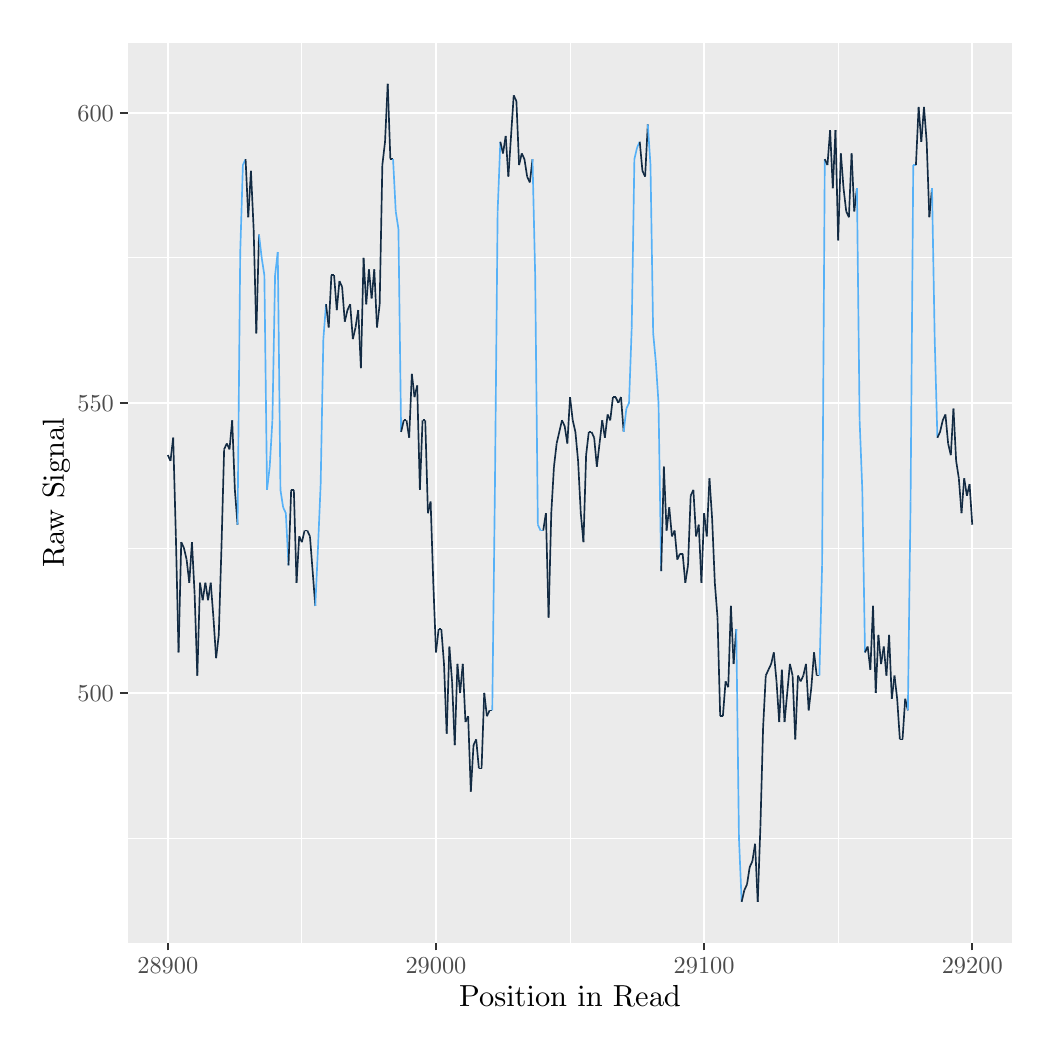
\begin{tikzpicture}[x=1pt,y=1pt]
\definecolor{fillColor}{RGB}{255,255,255}
\path[use as bounding box,fill=fillColor,fill opacity=0.00] (0,0) rectangle (361.35,361.35);
\begin{scope}
\path[clip] (  0.00,  0.00) rectangle (361.35,361.35);
\definecolor{drawColor}{RGB}{255,255,255}
\definecolor{fillColor}{RGB}{255,255,255}

\path[draw=drawColor,line width= 0.6pt,line join=round,line cap=round,fill=fillColor] (  0.00,  0.00) rectangle (361.35,361.35);
\end{scope}
\begin{scope}
\path[clip] ( 36.11, 30.69) rectangle (355.85,355.85);
\definecolor{fillColor}{gray}{0.92}

\path[fill=fillColor] ( 36.11, 30.69) rectangle (355.85,355.85);
\definecolor{drawColor}{RGB}{255,255,255}

\path[draw=drawColor,line width= 0.3pt,line join=round] ( 36.11, 68.53) --
	(355.85, 68.53);

\path[draw=drawColor,line width= 0.3pt,line join=round] ( 36.11,173.35) --
	(355.85,173.35);

\path[draw=drawColor,line width= 0.3pt,line join=round] ( 36.11,278.18) --
	(355.85,278.18);

\path[draw=drawColor,line width= 0.3pt,line join=round] ( 99.09, 30.69) --
	( 99.09,355.85);

\path[draw=drawColor,line width= 0.3pt,line join=round] (195.98, 30.69) --
	(195.98,355.85);

\path[draw=drawColor,line width= 0.3pt,line join=round] (292.87, 30.69) --
	(292.87,355.85);

\path[draw=drawColor,line width= 0.6pt,line join=round] ( 36.11,120.94) --
	(355.85,120.94);

\path[draw=drawColor,line width= 0.6pt,line join=round] ( 36.11,225.76) --
	(355.85,225.76);

\path[draw=drawColor,line width= 0.6pt,line join=round] ( 36.11,330.59) --
	(355.85,330.59);

\path[draw=drawColor,line width= 0.6pt,line join=round] ( 50.64, 30.69) --
	( 50.64,355.85);

\path[draw=drawColor,line width= 0.6pt,line join=round] (147.54, 30.69) --
	(147.54,355.85);

\path[draw=drawColor,line width= 0.6pt,line join=round] (244.43, 30.69) --
	(244.43,355.85);

\path[draw=drawColor,line width= 0.6pt,line join=round] (341.32, 30.69) --
	(341.32,355.85);
\definecolor{drawColor}{RGB}{19,43,67}

\path[draw=drawColor,line width= 0.6pt,line join=round] ( 50.64,206.90) -- ( 51.61,204.80);

\path[draw=drawColor,line width= 0.6pt,line join=round] ( 51.61,204.80) -- ( 52.58,213.18);

\path[draw=drawColor,line width= 0.6pt,line join=round] ( 52.58,213.18) -- ( 53.55,177.54);

\path[draw=drawColor,line width= 0.6pt,line join=round] ( 53.55,177.54) -- ( 54.52,135.61);

\path[draw=drawColor,line width= 0.6pt,line join=round] ( 54.52,135.61) -- ( 55.49,175.45);

\path[draw=drawColor,line width= 0.6pt,line join=round] ( 55.49,175.45) -- ( 56.46,173.35);

\path[draw=drawColor,line width= 0.6pt,line join=round] ( 56.46,173.35) -- ( 57.43,169.16);

\path[draw=drawColor,line width= 0.6pt,line join=round] ( 57.43,169.16) -- ( 58.40,160.77);

\path[draw=drawColor,line width= 0.6pt,line join=round] ( 58.40,160.77) -- ( 59.36,175.45);

\path[draw=drawColor,line width= 0.6pt,line join=round] ( 59.36,175.45) -- ( 60.33,156.58);

\path[draw=drawColor,line width= 0.6pt,line join=round] ( 60.33,156.58) -- ( 61.30,127.23);

\path[draw=drawColor,line width= 0.6pt,line join=round] ( 61.30,127.23) -- ( 62.27,160.77);

\path[draw=drawColor,line width= 0.6pt,line join=round] ( 62.27,160.77) -- ( 63.24,154.48);

\path[draw=drawColor,line width= 0.6pt,line join=round] ( 63.24,154.48) -- ( 64.21,160.77);

\path[draw=drawColor,line width= 0.6pt,line join=round] ( 64.21,160.77) -- ( 65.18,154.48);

\path[draw=drawColor,line width= 0.6pt,line join=round] ( 65.18,154.48) -- ( 66.15,160.77);

\path[draw=drawColor,line width= 0.6pt,line join=round] ( 66.15,160.77) -- ( 67.12,148.19);

\path[draw=drawColor,line width= 0.6pt,line join=round] ( 67.12,148.19) -- ( 68.09,133.52);

\path[draw=drawColor,line width= 0.6pt,line join=round] ( 68.09,133.52) -- ( 69.05,141.90);

\path[draw=drawColor,line width= 0.6pt,line join=round] ( 69.05,141.90) -- ( 70.02,173.35);

\path[draw=drawColor,line width= 0.6pt,line join=round] ( 70.02,173.35) -- ( 70.99,208.99);

\path[draw=drawColor,line width= 0.6pt,line join=round] ( 70.99,208.99) -- ( 71.96,211.09);

\path[draw=drawColor,line width= 0.6pt,line join=round] ( 71.96,211.09) -- ( 72.93,208.99);

\path[draw=drawColor,line width= 0.6pt,line join=round] ( 72.93,208.99) -- ( 73.90,219.47);

\path[draw=drawColor,line width= 0.6pt,line join=round] ( 73.90,219.47) -- ( 74.87,194.32);

\path[draw=drawColor,line width= 0.6pt,line join=round] ( 74.87,194.32) -- ( 75.84,181.74);
\definecolor{drawColor}{RGB}{86,177,247}

\path[draw=drawColor,line width= 0.6pt,line join=round] ( 75.84,181.74) -- ( 76.81,280.27);

\path[draw=drawColor,line width= 0.6pt,line join=round] ( 76.81,280.27) -- ( 77.77,311.72);

\path[draw=drawColor,line width= 0.6pt,line join=round] ( 77.77,311.72) -- ( 78.74,313.82);
\definecolor{drawColor}{RGB}{19,43,67}

\path[draw=drawColor,line width= 0.6pt,line join=round] ( 78.74,313.82) -- ( 79.71,292.85);

\path[draw=drawColor,line width= 0.6pt,line join=round] ( 79.71,292.85) -- ( 80.68,309.62);

\path[draw=drawColor,line width= 0.6pt,line join=round] ( 80.68,309.62) -- ( 81.65,288.66);

\path[draw=drawColor,line width= 0.6pt,line join=round] ( 81.65,288.66) -- ( 82.62,250.92);

\path[draw=drawColor,line width= 0.6pt,line join=round] ( 82.62,250.92) -- ( 83.59,286.56);
\definecolor{drawColor}{RGB}{86,177,247}

\path[draw=drawColor,line width= 0.6pt,line join=round] ( 83.59,286.56) -- ( 84.56,278.18);

\path[draw=drawColor,line width= 0.6pt,line join=round] ( 84.56,278.18) -- ( 85.53,271.89);

\path[draw=drawColor,line width= 0.6pt,line join=round] ( 85.53,271.89) -- ( 86.49,194.32);

\path[draw=drawColor,line width= 0.6pt,line join=round] ( 86.49,194.32) -- ( 87.46,202.70);

\path[draw=drawColor,line width= 0.6pt,line join=round] ( 87.46,202.70) -- ( 88.43,219.47);

\path[draw=drawColor,line width= 0.6pt,line join=round] ( 88.43,219.47) -- ( 89.40,271.89);

\path[draw=drawColor,line width= 0.6pt,line join=round] ( 89.40,271.89) -- ( 90.37,280.27);

\path[draw=drawColor,line width= 0.6pt,line join=round] ( 90.37,280.27) -- ( 91.34,194.32);

\path[draw=drawColor,line width= 0.6pt,line join=round] ( 91.34,194.32) -- ( 92.31,188.03);

\path[draw=drawColor,line width= 0.6pt,line join=round] ( 92.31,188.03) -- ( 93.28,185.93);

\path[draw=drawColor,line width= 0.6pt,line join=round] ( 93.28,185.93) -- ( 94.25,167.06);
\definecolor{drawColor}{RGB}{19,43,67}

\path[draw=drawColor,line width= 0.6pt,line join=round] ( 94.25,167.06) -- ( 95.21,194.32);

\path[draw=drawColor,line width= 0.6pt,line join=round] ( 95.21,194.32) -- ( 96.18,194.32);

\path[draw=drawColor,line width= 0.6pt,line join=round] ( 96.18,194.32) -- ( 97.15,160.77);

\path[draw=drawColor,line width= 0.6pt,line join=round] ( 97.15,160.77) -- ( 98.12,177.54);

\path[draw=drawColor,line width= 0.6pt,line join=round] ( 98.12,177.54) -- ( 99.09,175.45);

\path[draw=drawColor,line width= 0.6pt,line join=round] ( 99.09,175.45) -- (100.06,179.64);

\path[draw=drawColor,line width= 0.6pt,line join=round] (100.06,179.64) -- (101.03,179.64);

\path[draw=drawColor,line width= 0.6pt,line join=round] (101.03,179.64) -- (102.00,177.54);

\path[draw=drawColor,line width= 0.6pt,line join=round] (102.00,177.54) -- (102.97,164.97);

\path[draw=drawColor,line width= 0.6pt,line join=round] (102.97,164.97) -- (103.93,152.39);
\definecolor{drawColor}{RGB}{86,177,247}

\path[draw=drawColor,line width= 0.6pt,line join=round] (103.93,152.39) -- (104.90,173.35);

\path[draw=drawColor,line width= 0.6pt,line join=round] (104.90,173.35) -- (105.87,196.41);

\path[draw=drawColor,line width= 0.6pt,line join=round] (105.87,196.41) -- (106.84,248.82);

\path[draw=drawColor,line width= 0.6pt,line join=round] (106.84,248.82) -- (107.81,261.40);
\definecolor{drawColor}{RGB}{19,43,67}

\path[draw=drawColor,line width= 0.6pt,line join=round] (107.81,261.40) -- (108.78,253.02);

\path[draw=drawColor,line width= 0.6pt,line join=round] (108.78,253.02) -- (109.75,271.89);

\path[draw=drawColor,line width= 0.6pt,line join=round] (109.75,271.89) -- (110.72,271.89);

\path[draw=drawColor,line width= 0.6pt,line join=round] (110.72,271.89) -- (111.69,259.31);

\path[draw=drawColor,line width= 0.6pt,line join=round] (111.69,259.31) -- (112.65,269.79);

\path[draw=drawColor,line width= 0.6pt,line join=round] (112.65,269.79) -- (113.62,267.69);

\path[draw=drawColor,line width= 0.6pt,line join=round] (113.62,267.69) -- (114.59,255.11);

\path[draw=drawColor,line width= 0.6pt,line join=round] (114.59,255.11) -- (115.56,259.31);

\path[draw=drawColor,line width= 0.6pt,line join=round] (115.56,259.31) -- (116.53,261.40);

\path[draw=drawColor,line width= 0.6pt,line join=round] (116.53,261.40) -- (117.50,248.82);

\path[draw=drawColor,line width= 0.6pt,line join=round] (117.50,248.82) -- (118.47,253.02);

\path[draw=drawColor,line width= 0.6pt,line join=round] (118.47,253.02) -- (119.44,259.31);

\path[draw=drawColor,line width= 0.6pt,line join=round] (119.44,259.31) -- (120.41,238.34);

\path[draw=drawColor,line width= 0.6pt,line join=round] (120.41,238.34) -- (121.37,278.18);

\path[draw=drawColor,line width= 0.6pt,line join=round] (121.37,278.18) -- (122.34,261.40);

\path[draw=drawColor,line width= 0.6pt,line join=round] (122.34,261.40) -- (123.31,273.98);

\path[draw=drawColor,line width= 0.6pt,line join=round] (123.31,273.98) -- (124.28,263.50);

\path[draw=drawColor,line width= 0.6pt,line join=round] (124.28,263.50) -- (125.25,273.98);

\path[draw=drawColor,line width= 0.6pt,line join=round] (125.25,273.98) -- (126.22,253.02);

\path[draw=drawColor,line width= 0.6pt,line join=round] (126.22,253.02) -- (127.19,261.40);

\path[draw=drawColor,line width= 0.6pt,line join=round] (127.19,261.40) -- (128.16,311.72);

\path[draw=drawColor,line width= 0.6pt,line join=round] (128.16,311.72) -- (129.13,320.11);

\path[draw=drawColor,line width= 0.6pt,line join=round] (129.13,320.11) -- (130.10,341.07);

\path[draw=drawColor,line width= 0.6pt,line join=round] (130.10,341.07) -- (131.06,313.82);

\path[draw=drawColor,line width= 0.6pt,line join=round] (131.06,313.82) -- (132.03,313.82);
\definecolor{drawColor}{RGB}{86,177,247}

\path[draw=drawColor,line width= 0.6pt,line join=round] (132.03,313.82) -- (133.00,294.95);

\path[draw=drawColor,line width= 0.6pt,line join=round] (133.00,294.95) -- (133.97,288.66);

\path[draw=drawColor,line width= 0.6pt,line join=round] (133.97,288.66) -- (134.94,215.28);
\definecolor{drawColor}{RGB}{19,43,67}

\path[draw=drawColor,line width= 0.6pt,line join=round] (134.94,215.28) -- (135.91,219.47);

\path[draw=drawColor,line width= 0.6pt,line join=round] (135.91,219.47) -- (136.88,219.47);

\path[draw=drawColor,line width= 0.6pt,line join=round] (136.88,219.47) -- (137.85,213.18);

\path[draw=drawColor,line width= 0.6pt,line join=round] (137.85,213.18) -- (138.82,236.25);

\path[draw=drawColor,line width= 0.6pt,line join=round] (138.82,236.25) -- (139.78,227.86);

\path[draw=drawColor,line width= 0.6pt,line join=round] (139.78,227.86) -- (140.75,232.05);

\path[draw=drawColor,line width= 0.6pt,line join=round] (140.75,232.05) -- (141.72,194.32);

\path[draw=drawColor,line width= 0.6pt,line join=round] (141.72,194.32) -- (142.69,219.47);

\path[draw=drawColor,line width= 0.6pt,line join=round] (142.69,219.47) -- (143.66,219.47);

\path[draw=drawColor,line width= 0.6pt,line join=round] (143.66,219.47) -- (144.63,185.93);

\path[draw=drawColor,line width= 0.6pt,line join=round] (144.63,185.93) -- (145.60,190.12);

\path[draw=drawColor,line width= 0.6pt,line join=round] (145.60,190.12) -- (146.57,160.77);

\path[draw=drawColor,line width= 0.6pt,line join=round] (146.57,160.77) -- (147.54,135.61);

\path[draw=drawColor,line width= 0.6pt,line join=round] (147.54,135.61) -- (148.50,144.00);

\path[draw=drawColor,line width= 0.6pt,line join=round] (148.50,144.00) -- (149.47,144.00);

\path[draw=drawColor,line width= 0.6pt,line join=round] (149.47,144.00) -- (150.44,131.42);

\path[draw=drawColor,line width= 0.6pt,line join=round] (150.44,131.42) -- (151.41,106.26);

\path[draw=drawColor,line width= 0.6pt,line join=round] (151.41,106.26) -- (152.38,137.71);

\path[draw=drawColor,line width= 0.6pt,line join=round] (152.38,137.71) -- (153.35,125.13);

\path[draw=drawColor,line width= 0.6pt,line join=round] (153.35,125.13) -- (154.32,102.07);

\path[draw=drawColor,line width= 0.6pt,line join=round] (154.32,102.07) -- (155.29,131.42);

\path[draw=drawColor,line width= 0.6pt,line join=round] (155.29,131.42) -- (156.26,120.94);

\path[draw=drawColor,line width= 0.6pt,line join=round] (156.26,120.94) -- (157.22,131.42);

\path[draw=drawColor,line width= 0.6pt,line join=round] (157.22,131.42) -- (158.19,110.46);

\path[draw=drawColor,line width= 0.6pt,line join=round] (158.19,110.46) -- (159.16,112.55);

\path[draw=drawColor,line width= 0.6pt,line join=round] (159.16,112.55) -- (160.13, 85.30);

\path[draw=drawColor,line width= 0.6pt,line join=round] (160.13, 85.30) -- (161.10,102.07);

\path[draw=drawColor,line width= 0.6pt,line join=round] (161.10,102.07) -- (162.07,104.17);

\path[draw=drawColor,line width= 0.6pt,line join=round] (162.07,104.17) -- (163.04, 93.69);

\path[draw=drawColor,line width= 0.6pt,line join=round] (163.04, 93.69) -- (164.01, 93.69);

\path[draw=drawColor,line width= 0.6pt,line join=round] (164.01, 93.69) -- (164.98,120.94);

\path[draw=drawColor,line width= 0.6pt,line join=round] (164.98,120.94) -- (165.94,112.55);

\path[draw=drawColor,line width= 0.6pt,line join=round] (165.94,112.55) -- (166.91,114.65);

\path[draw=drawColor,line width= 0.6pt,line join=round] (166.91,114.65) -- (167.88,114.65);
\definecolor{drawColor}{RGB}{86,177,247}

\path[draw=drawColor,line width= 0.6pt,line join=round] (167.88,114.65) -- (168.85,196.41);

\path[draw=drawColor,line width= 0.6pt,line join=round] (168.85,196.41) -- (169.82,294.95);

\path[draw=drawColor,line width= 0.6pt,line join=round] (169.82,294.95) -- (170.79,320.11);
\definecolor{drawColor}{RGB}{19,43,67}

\path[draw=drawColor,line width= 0.6pt,line join=round] (170.79,320.11) -- (171.76,315.91);

\path[draw=drawColor,line width= 0.6pt,line join=round] (171.76,315.91) -- (172.73,322.20);

\path[draw=drawColor,line width= 0.6pt,line join=round] (172.73,322.20) -- (173.70,307.53);

\path[draw=drawColor,line width= 0.6pt,line join=round] (173.70,307.53) -- (174.66,322.20);

\path[draw=drawColor,line width= 0.6pt,line join=round] (174.66,322.20) -- (175.63,336.88);

\path[draw=drawColor,line width= 0.6pt,line join=round] (175.63,336.88) -- (176.60,334.78);

\path[draw=drawColor,line width= 0.6pt,line join=round] (176.60,334.78) -- (177.57,311.72);

\path[draw=drawColor,line width= 0.6pt,line join=round] (177.57,311.72) -- (178.54,315.91);

\path[draw=drawColor,line width= 0.6pt,line join=round] (178.54,315.91) -- (179.51,313.82);

\path[draw=drawColor,line width= 0.6pt,line join=round] (179.51,313.82) -- (180.48,307.53);

\path[draw=drawColor,line width= 0.6pt,line join=round] (180.48,307.53) -- (181.45,305.43);

\path[draw=drawColor,line width= 0.6pt,line join=round] (181.45,305.43) -- (182.42,313.82);
\definecolor{drawColor}{RGB}{86,177,247}

\path[draw=drawColor,line width= 0.6pt,line join=round] (182.42,313.82) -- (183.38,271.89);

\path[draw=drawColor,line width= 0.6pt,line join=round] (183.38,271.89) -- (184.35,181.74);

\path[draw=drawColor,line width= 0.6pt,line join=round] (184.35,181.74) -- (185.32,179.64);

\path[draw=drawColor,line width= 0.6pt,line join=round] (185.32,179.64) -- (186.29,179.64);
\definecolor{drawColor}{RGB}{19,43,67}

\path[draw=drawColor,line width= 0.6pt,line join=round] (186.29,179.64) -- (187.26,185.93);

\path[draw=drawColor,line width= 0.6pt,line join=round] (187.26,185.93) -- (188.23,148.19);

\path[draw=drawColor,line width= 0.6pt,line join=round] (188.23,148.19) -- (189.20,185.93);

\path[draw=drawColor,line width= 0.6pt,line join=round] (189.20,185.93) -- (190.17,202.70);

\path[draw=drawColor,line width= 0.6pt,line join=round] (190.17,202.70) -- (191.14,211.09);

\path[draw=drawColor,line width= 0.6pt,line join=round] (191.14,211.09) -- (192.10,215.28);

\path[draw=drawColor,line width= 0.6pt,line join=round] (192.10,215.28) -- (193.07,219.47);

\path[draw=drawColor,line width= 0.6pt,line join=round] (193.07,219.47) -- (194.04,217.38);

\path[draw=drawColor,line width= 0.6pt,line join=round] (194.04,217.38) -- (195.01,211.09);

\path[draw=drawColor,line width= 0.6pt,line join=round] (195.01,211.09) -- (195.98,227.86);

\path[draw=drawColor,line width= 0.6pt,line join=round] (195.98,227.86) -- (196.95,219.47);

\path[draw=drawColor,line width= 0.6pt,line join=round] (196.95,219.47) -- (197.92,215.28);

\path[draw=drawColor,line width= 0.6pt,line join=round] (197.92,215.28) -- (198.89,204.80);

\path[draw=drawColor,line width= 0.6pt,line join=round] (198.89,204.80) -- (199.86,185.93);

\path[draw=drawColor,line width= 0.6pt,line join=round] (199.86,185.93) -- (200.83,175.45);

\path[draw=drawColor,line width= 0.6pt,line join=round] (200.83,175.45) -- (201.79,206.90);

\path[draw=drawColor,line width= 0.6pt,line join=round] (201.79,206.90) -- (202.76,215.28);

\path[draw=drawColor,line width= 0.6pt,line join=round] (202.76,215.28) -- (203.73,215.28);

\path[draw=drawColor,line width= 0.6pt,line join=round] (203.73,215.28) -- (204.70,213.18);

\path[draw=drawColor,line width= 0.6pt,line join=round] (204.70,213.18) -- (205.67,202.70);

\path[draw=drawColor,line width= 0.6pt,line join=round] (205.67,202.70) -- (206.64,211.09);

\path[draw=drawColor,line width= 0.6pt,line join=round] (206.64,211.09) -- (207.61,219.47);

\path[draw=drawColor,line width= 0.6pt,line join=round] (207.61,219.47) -- (208.58,213.18);

\path[draw=drawColor,line width= 0.6pt,line join=round] (208.58,213.18) -- (209.55,221.57);

\path[draw=drawColor,line width= 0.6pt,line join=round] (209.55,221.57) -- (210.51,219.47);

\path[draw=drawColor,line width= 0.6pt,line join=round] (210.51,219.47) -- (211.48,227.86);

\path[draw=drawColor,line width= 0.6pt,line join=round] (211.48,227.86) -- (212.45,227.86);

\path[draw=drawColor,line width= 0.6pt,line join=round] (212.45,227.86) -- (213.42,225.76);

\path[draw=drawColor,line width= 0.6pt,line join=round] (213.42,225.76) -- (214.39,227.86);

\path[draw=drawColor,line width= 0.6pt,line join=round] (214.39,227.86) -- (215.36,215.28);
\definecolor{drawColor}{RGB}{86,177,247}

\path[draw=drawColor,line width= 0.6pt,line join=round] (215.36,215.28) -- (216.33,223.67);

\path[draw=drawColor,line width= 0.6pt,line join=round] (216.33,223.67) -- (217.30,225.76);

\path[draw=drawColor,line width= 0.6pt,line join=round] (217.30,225.76) -- (218.27,253.02);

\path[draw=drawColor,line width= 0.6pt,line join=round] (218.27,253.02) -- (219.23,313.82);

\path[draw=drawColor,line width= 0.6pt,line join=round] (219.23,313.82) -- (220.20,318.01);

\path[draw=drawColor,line width= 0.6pt,line join=round] (220.20,318.01) -- (221.17,320.11);
\definecolor{drawColor}{RGB}{19,43,67}

\path[draw=drawColor,line width= 0.6pt,line join=round] (221.17,320.11) -- (222.14,309.62);

\path[draw=drawColor,line width= 0.6pt,line join=round] (222.14,309.62) -- (223.11,307.53);

\path[draw=drawColor,line width= 0.6pt,line join=round] (223.11,307.53) -- (224.08,326.39);
\definecolor{drawColor}{RGB}{86,177,247}

\path[draw=drawColor,line width= 0.6pt,line join=round] (224.08,326.39) -- (225.05,311.72);

\path[draw=drawColor,line width= 0.6pt,line join=round] (225.05,311.72) -- (226.02,250.92);

\path[draw=drawColor,line width= 0.6pt,line join=round] (226.02,250.92) -- (226.99,240.44);

\path[draw=drawColor,line width= 0.6pt,line join=round] (226.99,240.44) -- (227.95,225.76);

\path[draw=drawColor,line width= 0.6pt,line join=round] (227.95,225.76) -- (228.92,164.97);
\definecolor{drawColor}{RGB}{19,43,67}

\path[draw=drawColor,line width= 0.6pt,line join=round] (228.92,164.97) -- (229.89,202.70);

\path[draw=drawColor,line width= 0.6pt,line join=round] (229.89,202.70) -- (230.86,179.64);

\path[draw=drawColor,line width= 0.6pt,line join=round] (230.86,179.64) -- (231.83,188.03);

\path[draw=drawColor,line width= 0.6pt,line join=round] (231.83,188.03) -- (232.80,177.54);

\path[draw=drawColor,line width= 0.6pt,line join=round] (232.80,177.54) -- (233.77,179.64);

\path[draw=drawColor,line width= 0.6pt,line join=round] (233.77,179.64) -- (234.74,169.16);

\path[draw=drawColor,line width= 0.6pt,line join=round] (234.74,169.16) -- (235.71,171.25);

\path[draw=drawColor,line width= 0.6pt,line join=round] (235.71,171.25) -- (236.67,171.25);

\path[draw=drawColor,line width= 0.6pt,line join=round] (236.67,171.25) -- (237.64,160.77);

\path[draw=drawColor,line width= 0.6pt,line join=round] (237.64,160.77) -- (238.61,167.06);

\path[draw=drawColor,line width= 0.6pt,line join=round] (238.61,167.06) -- (239.58,192.22);

\path[draw=drawColor,line width= 0.6pt,line join=round] (239.58,192.22) -- (240.55,194.32);

\path[draw=drawColor,line width= 0.6pt,line join=round] (240.55,194.32) -- (241.52,177.54);

\path[draw=drawColor,line width= 0.6pt,line join=round] (241.52,177.54) -- (242.49,181.74);

\path[draw=drawColor,line width= 0.6pt,line join=round] (242.49,181.74) -- (243.46,160.77);

\path[draw=drawColor,line width= 0.6pt,line join=round] (243.46,160.77) -- (244.43,185.93);

\path[draw=drawColor,line width= 0.6pt,line join=round] (244.43,185.93) -- (245.39,177.54);

\path[draw=drawColor,line width= 0.6pt,line join=round] (245.39,177.54) -- (246.36,198.51);

\path[draw=drawColor,line width= 0.6pt,line join=round] (246.36,198.51) -- (247.33,183.83);

\path[draw=drawColor,line width= 0.6pt,line join=round] (247.33,183.83) -- (248.30,160.77);

\path[draw=drawColor,line width= 0.6pt,line join=round] (248.30,160.77) -- (249.27,148.19);

\path[draw=drawColor,line width= 0.6pt,line join=round] (249.27,148.19) -- (250.24,112.55);

\path[draw=drawColor,line width= 0.6pt,line join=round] (250.24,112.55) -- (251.21,112.55);

\path[draw=drawColor,line width= 0.6pt,line join=round] (251.21,112.55) -- (252.18,125.13);

\path[draw=drawColor,line width= 0.6pt,line join=round] (252.18,125.13) -- (253.15,123.04);

\path[draw=drawColor,line width= 0.6pt,line join=round] (253.15,123.04) -- (254.11,152.39);

\path[draw=drawColor,line width= 0.6pt,line join=round] (254.11,152.39) -- (255.08,131.42);

\path[draw=drawColor,line width= 0.6pt,line join=round] (255.08,131.42) -- (256.05,144.00);
\definecolor{drawColor}{RGB}{86,177,247}

\path[draw=drawColor,line width= 0.6pt,line join=round] (256.05,144.00) -- (257.02, 68.53);

\path[draw=drawColor,line width= 0.6pt,line join=round] (257.02, 68.53) -- (257.99, 45.47);
\definecolor{drawColor}{RGB}{19,43,67}

\path[draw=drawColor,line width= 0.6pt,line join=round] (257.99, 45.47) -- (258.96, 49.66);

\path[draw=drawColor,line width= 0.6pt,line join=round] (258.96, 49.66) -- (259.93, 51.76);

\path[draw=drawColor,line width= 0.6pt,line join=round] (259.93, 51.76) -- (260.90, 58.04);

\path[draw=drawColor,line width= 0.6pt,line join=round] (260.90, 58.04) -- (261.87, 60.14);

\path[draw=drawColor,line width= 0.6pt,line join=round] (261.87, 60.14) -- (262.84, 66.43);

\path[draw=drawColor,line width= 0.6pt,line join=round] (262.84, 66.43) -- (263.80, 45.47);

\path[draw=drawColor,line width= 0.6pt,line join=round] (263.80, 45.47) -- (264.77, 72.72);

\path[draw=drawColor,line width= 0.6pt,line join=round] (264.77, 72.72) -- (265.74,108.36);

\path[draw=drawColor,line width= 0.6pt,line join=round] (265.74,108.36) -- (266.71,127.23);

\path[draw=drawColor,line width= 0.6pt,line join=round] (266.71,127.23) -- (267.68,129.33);

\path[draw=drawColor,line width= 0.6pt,line join=round] (267.68,129.33) -- (268.65,131.42);

\path[draw=drawColor,line width= 0.6pt,line join=round] (268.65,131.42) -- (269.62,135.61);

\path[draw=drawColor,line width= 0.6pt,line join=round] (269.62,135.61) -- (270.59,125.13);

\path[draw=drawColor,line width= 0.6pt,line join=round] (270.59,125.13) -- (271.56,110.46);

\path[draw=drawColor,line width= 0.6pt,line join=round] (271.56,110.46) -- (272.52,129.33);

\path[draw=drawColor,line width= 0.6pt,line join=round] (272.52,129.33) -- (273.49,110.46);

\path[draw=drawColor,line width= 0.6pt,line join=round] (273.49,110.46) -- (274.46,120.94);

\path[draw=drawColor,line width= 0.6pt,line join=round] (274.46,120.94) -- (275.43,131.42);

\path[draw=drawColor,line width= 0.6pt,line join=round] (275.43,131.42) -- (276.40,127.23);

\path[draw=drawColor,line width= 0.6pt,line join=round] (276.40,127.23) -- (277.37,104.17);

\path[draw=drawColor,line width= 0.6pt,line join=round] (277.37,104.17) -- (278.34,127.23);

\path[draw=drawColor,line width= 0.6pt,line join=round] (278.34,127.23) -- (279.31,125.13);

\path[draw=drawColor,line width= 0.6pt,line join=round] (279.31,125.13) -- (280.28,127.23);

\path[draw=drawColor,line width= 0.6pt,line join=round] (280.28,127.23) -- (281.24,131.42);

\path[draw=drawColor,line width= 0.6pt,line join=round] (281.24,131.42) -- (282.21,114.65);

\path[draw=drawColor,line width= 0.6pt,line join=round] (282.21,114.65) -- (283.18,123.04);

\path[draw=drawColor,line width= 0.6pt,line join=round] (283.18,123.04) -- (284.15,135.61);

\path[draw=drawColor,line width= 0.6pt,line join=round] (284.15,135.61) -- (285.12,127.23);

\path[draw=drawColor,line width= 0.6pt,line join=round] (285.12,127.23) -- (286.09,127.23);
\definecolor{drawColor}{RGB}{86,177,247}

\path[draw=drawColor,line width= 0.6pt,line join=round] (286.09,127.23) -- (287.06,167.06);

\path[draw=drawColor,line width= 0.6pt,line join=round] (287.06,167.06) -- (288.03,313.82);
\definecolor{drawColor}{RGB}{19,43,67}

\path[draw=drawColor,line width= 0.6pt,line join=round] (288.03,313.82) -- (289.00,311.72);

\path[draw=drawColor,line width= 0.6pt,line join=round] (289.00,311.72) -- (289.96,324.30);

\path[draw=drawColor,line width= 0.6pt,line join=round] (289.96,324.30) -- (290.93,303.33);

\path[draw=drawColor,line width= 0.6pt,line join=round] (290.93,303.33) -- (291.90,324.30);

\path[draw=drawColor,line width= 0.6pt,line join=round] (291.90,324.30) -- (292.87,284.46);

\path[draw=drawColor,line width= 0.6pt,line join=round] (292.87,284.46) -- (293.84,315.91);

\path[draw=drawColor,line width= 0.6pt,line join=round] (293.84,315.91) -- (294.81,303.33);

\path[draw=drawColor,line width= 0.6pt,line join=round] (294.81,303.33) -- (295.78,294.95);

\path[draw=drawColor,line width= 0.6pt,line join=round] (295.78,294.95) -- (296.75,292.85);

\path[draw=drawColor,line width= 0.6pt,line join=round] (296.75,292.85) -- (297.72,315.91);

\path[draw=drawColor,line width= 0.6pt,line join=round] (297.72,315.91) -- (298.68,294.95);

\path[draw=drawColor,line width= 0.6pt,line join=round] (298.68,294.95) -- (299.65,303.33);
\definecolor{drawColor}{RGB}{86,177,247}

\path[draw=drawColor,line width= 0.6pt,line join=round] (299.65,303.33) -- (300.62,219.47);

\path[draw=drawColor,line width= 0.6pt,line join=round] (300.62,219.47) -- (301.59,194.32);

\path[draw=drawColor,line width= 0.6pt,line join=round] (301.59,194.32) -- (302.56,135.61);
\definecolor{drawColor}{RGB}{19,43,67}

\path[draw=drawColor,line width= 0.6pt,line join=round] (302.56,135.61) -- (303.53,137.71);

\path[draw=drawColor,line width= 0.6pt,line join=round] (303.53,137.71) -- (304.50,129.33);

\path[draw=drawColor,line width= 0.6pt,line join=round] (304.50,129.33) -- (305.47,152.39);

\path[draw=drawColor,line width= 0.6pt,line join=round] (305.47,152.39) -- (306.44,120.94);

\path[draw=drawColor,line width= 0.6pt,line join=round] (306.44,120.94) -- (307.40,141.90);

\path[draw=drawColor,line width= 0.6pt,line join=round] (307.40,141.90) -- (308.37,131.42);

\path[draw=drawColor,line width= 0.6pt,line join=round] (308.37,131.42) -- (309.34,137.71);

\path[draw=drawColor,line width= 0.6pt,line join=round] (309.34,137.71) -- (310.31,127.23);

\path[draw=drawColor,line width= 0.6pt,line join=round] (310.31,127.23) -- (311.28,141.90);

\path[draw=drawColor,line width= 0.6pt,line join=round] (311.28,141.90) -- (312.25,118.84);

\path[draw=drawColor,line width= 0.6pt,line join=round] (312.25,118.84) -- (313.22,127.23);

\path[draw=drawColor,line width= 0.6pt,line join=round] (313.22,127.23) -- (314.19,118.84);

\path[draw=drawColor,line width= 0.6pt,line join=round] (314.19,118.84) -- (315.16,104.17);

\path[draw=drawColor,line width= 0.6pt,line join=round] (315.16,104.17) -- (316.12,104.17);

\path[draw=drawColor,line width= 0.6pt,line join=round] (316.12,104.17) -- (317.09,118.84);

\path[draw=drawColor,line width= 0.6pt,line join=round] (317.09,118.84) -- (318.06,114.65);
\definecolor{drawColor}{RGB}{86,177,247}

\path[draw=drawColor,line width= 0.6pt,line join=round] (318.06,114.65) -- (319.03,190.12);

\path[draw=drawColor,line width= 0.6pt,line join=round] (319.03,190.12) -- (320.00,311.72);

\path[draw=drawColor,line width= 0.6pt,line join=round] (320.00,311.72) -- (320.97,311.72);
\definecolor{drawColor}{RGB}{19,43,67}

\path[draw=drawColor,line width= 0.6pt,line join=round] (320.97,311.72) -- (321.94,332.68);

\path[draw=drawColor,line width= 0.6pt,line join=round] (321.94,332.68) -- (322.91,320.11);

\path[draw=drawColor,line width= 0.6pt,line join=round] (322.91,320.11) -- (323.88,332.68);

\path[draw=drawColor,line width= 0.6pt,line join=round] (323.88,332.68) -- (324.85,320.11);

\path[draw=drawColor,line width= 0.6pt,line join=round] (324.85,320.11) -- (325.81,292.85);

\path[draw=drawColor,line width= 0.6pt,line join=round] (325.81,292.85) -- (326.78,303.33);
\definecolor{drawColor}{RGB}{86,177,247}

\path[draw=drawColor,line width= 0.6pt,line join=round] (326.78,303.33) -- (327.75,248.82);

\path[draw=drawColor,line width= 0.6pt,line join=round] (327.75,248.82) -- (328.72,213.18);
\definecolor{drawColor}{RGB}{19,43,67}

\path[draw=drawColor,line width= 0.6pt,line join=round] (328.72,213.18) -- (329.69,215.28);

\path[draw=drawColor,line width= 0.6pt,line join=round] (329.69,215.28) -- (330.66,219.47);

\path[draw=drawColor,line width= 0.6pt,line join=round] (330.66,219.47) -- (331.63,221.57);

\path[draw=drawColor,line width= 0.6pt,line join=round] (331.63,221.57) -- (332.60,211.09);

\path[draw=drawColor,line width= 0.6pt,line join=round] (332.60,211.09) -- (333.57,206.90);

\path[draw=drawColor,line width= 0.6pt,line join=round] (333.57,206.90) -- (334.53,223.67);

\path[draw=drawColor,line width= 0.6pt,line join=round] (334.53,223.67) -- (335.50,204.80);

\path[draw=drawColor,line width= 0.6pt,line join=round] (335.50,204.80) -- (336.47,198.51);

\path[draw=drawColor,line width= 0.6pt,line join=round] (336.47,198.51) -- (337.44,185.93);

\path[draw=drawColor,line width= 0.6pt,line join=round] (337.44,185.93) -- (338.41,198.51);

\path[draw=drawColor,line width= 0.6pt,line join=round] (338.41,198.51) -- (339.38,192.22);

\path[draw=drawColor,line width= 0.6pt,line join=round] (339.38,192.22) -- (340.35,196.41);

\path[draw=drawColor,line width= 0.6pt,line join=round] (340.35,196.41) -- (341.32,181.74);
\end{scope}
\begin{scope}
\path[clip] (  0.00,  0.00) rectangle (361.35,361.35);
\definecolor{drawColor}{gray}{0.30}

\node[text=drawColor,anchor=base east,inner sep=0pt, outer sep=0pt, scale=  0.88] at ( 31.16,117.91) {500};

\node[text=drawColor,anchor=base east,inner sep=0pt, outer sep=0pt, scale=  0.88] at ( 31.16,222.73) {550};

\node[text=drawColor,anchor=base east,inner sep=0pt, outer sep=0pt, scale=  0.88] at ( 31.16,327.56) {600};
\end{scope}
\begin{scope}
\path[clip] (  0.00,  0.00) rectangle (361.35,361.35);
\definecolor{drawColor}{gray}{0.20}

\path[draw=drawColor,line width= 0.6pt,line join=round] ( 33.36,120.94) --
	( 36.11,120.94);

\path[draw=drawColor,line width= 0.6pt,line join=round] ( 33.36,225.76) --
	( 36.11,225.76);

\path[draw=drawColor,line width= 0.6pt,line join=round] ( 33.36,330.59) --
	( 36.11,330.59);
\end{scope}
\begin{scope}
\path[clip] (  0.00,  0.00) rectangle (361.35,361.35);
\definecolor{drawColor}{gray}{0.20}

\path[draw=drawColor,line width= 0.6pt,line join=round] ( 50.64, 27.94) --
	( 50.64, 30.69);

\path[draw=drawColor,line width= 0.6pt,line join=round] (147.54, 27.94) --
	(147.54, 30.69);

\path[draw=drawColor,line width= 0.6pt,line join=round] (244.43, 27.94) --
	(244.43, 30.69);

\path[draw=drawColor,line width= 0.6pt,line join=round] (341.32, 27.94) --
	(341.32, 30.69);
\end{scope}
\begin{scope}
\path[clip] (  0.00,  0.00) rectangle (361.35,361.35);
\definecolor{drawColor}{gray}{0.30}

\node[text=drawColor,anchor=base,inner sep=0pt, outer sep=0pt, scale=  0.88] at ( 50.64, 19.68) {28900};

\node[text=drawColor,anchor=base,inner sep=0pt, outer sep=0pt, scale=  0.88] at (147.54, 19.68) {29000};

\node[text=drawColor,anchor=base,inner sep=0pt, outer sep=0pt, scale=  0.88] at (244.43, 19.68) {29100};

\node[text=drawColor,anchor=base,inner sep=0pt, outer sep=0pt, scale=  0.88] at (341.32, 19.68) {29200};
\end{scope}
\begin{scope}
\path[clip] (  0.00,  0.00) rectangle (361.35,361.35);
\definecolor{drawColor}{RGB}{0,0,0}

\node[text=drawColor,anchor=base,inner sep=0pt, outer sep=0pt, scale=  1.10] at (195.98,  7.64) {Position in Read};
\end{scope}
\begin{scope}
\path[clip] (  0.00,  0.00) rectangle (361.35,361.35);
\definecolor{drawColor}{RGB}{0,0,0}

\node[text=drawColor,rotate= 90.00,anchor=base,inner sep=0pt, outer sep=0pt, scale=  1.10] at ( 13.08,193.27) {Raw Signal};
\end{scope}
\end{tikzpicture}

\caption{\label{fig:epsilon-25}300 data points from a DNA section in the read with ID e9f08690-171f-476f-9119-5330d0290126. The jumps and falls are highlighted for $\epsilon=24$.}
\end{figure}


The \textit{jumps} encoding separates the two distributions by storing the number of
jumps and falls, the starting indices and lengths of the jumps and falls, the
absolute deltas of the jumps and falls, and finally the zig-zag deltas of the
flats. See Figure \ref{fig:jumps-enc} for more details. Since the deltas are
being encoded, the first point in the read must be recorded for invertibility.
Furthermore, because the falls have negative deltas, the absolute value of their
deltas is recorded. This means the jumps and falls deltas are all positive
whilst their distance from zero remains the same -- unlike what happens during
the zig-zag transformation where the data's distance from zero is roughly
doubled.

\begin{figure}
\centering\begin{tikzpicture}[node distance=0cm,start chain=1 going right,start chain=2 going right,start chain=3 going right] \footnotesize
  \tikzstyle{mytape}=[draw,minimum height=1.9cm]
	\node(A1)  [on chain=1,mytape,fill=yellow!20] {$\underset{\text{of jumps}}{\underbrace{\overbracket{n_j}^{\text{2 bytes}}}_{\text{number}}}$};
	\node(A2)  [on chain=1,mytape,fill=yellow!20] {$\underset{\text{of falls}}{\underbrace{\overbracket{n_f}^{\text{2 bytes}}}_{\text{number}}}$};
	\node(A3)  [on chain=1,mytape,fill=yellow!20] {$\underbrace{\overbracket{x_0}^{\text{2 bytes}}}_{\text{first point}}$};
	\node(B1)  [on chain=2,mytape,fill=green!20,below of=A1,xshift=0.98cm,node distance=1.9cm] {$\underset{\text{starting indices compressed size}}{\underbrace{\overbracket{m_p}^{\text{4 bytes}}}_{\text{jumps and falls}}}$};
	\node(B2)  [on chain=2,mytape,fill=green!35] {$\underset{\text{starting indices compressed data}}{\underbrace{\overbracket{C_{position}(p_{j_1},\dots,p_{j_{n_j}},p_{f_1},\dots,p_{f_{n_f}})}^{m_p\text{ bytes}}}_{\text{jumps and falls}}}$};
	\node(C1)  [on chain=3,mytape,fill=green!20,below of=B1,xshift=-0.335cm,node distance=1.9cm] {$\underset{\text{lengths compressed size}}{\underbrace{\overbracket{m_l}^{\text{4 bytes}}}_{\text{jumps and falls}}}$};
	\node(C2)  [on chain=3,mytape,fill=green!35] {$\underset{\text{lengths compressed data}}{\underbrace{\overbracket{C_{length}(|j_1|,\dots,|j_{n_j}|,|f_1|,\dots,|f_{n_f}|)}^{m_l\text{ bytes}}}_{\text{jumps and falls}}}$};
	\node(D1)  [on chain=4,mytape,fill=orange!20,below of=C1,xshift=-0.33cm,node distance=1.9cm] {$\underset{\text{compressed size}}{\underbrace{\overbracket{m_{jf}}^{\text{4 bytes}}}_{\text{jumps and falls}}}$};
	\node(D2)  [on chain=4,mytape,fill=orange!35] {$\underset{\text{compressed data}}{\underbrace{\overbracket{C_{jf}(\delta(j_1),\dots,\delta(j_{n_j}),-\delta(f_1),\dots,-\delta(f_{n_f}))}^{m_{jf}\text{ bytes}}}_{\text{jumps and falls}}}$};
	\node(E1)  [on chain=5,mytape,fill=red!20,below of=D1,xshift=0.2cm,node distance=1.9cm] {$\underbrace{\overbracket{m_{fl}}^{\text{4 bytes}}}_{\text{flats compressed size}}$};
	\node(E2)  [on chain=5,mytape,fill=red!35] {$\underbrace{\overbracket{C_{flats}(\delta(fl_1),\dots,\delta(fl_{n_{fl}}))}^{m_{fl}\text{ bytes}}}_{\text{flats compressed data}}$};
\end{tikzpicture}
	\caption{\label{fig:jumps-enc}The jumps encoding stores the number of
jumps and falls, and the first data point in the read since the deltas are being
encoded. The starting indices of the jumps and falls are compressed then their
lengths are compressed. Next, the deltas of the jumps and the negative deltas of
the falls are compressed together, followed by the deltas of the flats. There
are opportunities for four different compression techniques given the different
data streams.}
\end{figure}


A caveat with the jumps encoding is that the starting positions of the jumps and flats
must be recorded since the interleaving order of the jumps and flats is not
maintained. An alternative approach would be to take the zig-zag deltas of the
jumps and flats and maintain their order. In which case, recording the starting
positions would not be necessary since the order has been maintained in the
zig-zag deltas data stream. The length of jumps which are followed by falls and
vice-versa could then be represented by a place-holder such as zero since the
end of the jump would be marked by a negative delta. This works because a
jump/fall or flat will never have a length of zero. However, a new data stream
would need to be used to mark when a jump/fall and a flat occurs. Consider a bit
stream where 1 is a jump/fall and 0 is a flat. The interesting observation is
that since flats will always be preceded and followed by a jump/fall, 0 will
always be surrounded by 1s in the bit stream. This gives the potential for
a reasonable compression strategy on the bit stream. In addition, the length of each
flat would need to be recorded, such as by combining them with the lengths of
the jumps and falls. See Figure \ref{fig:jumps-enc-alt1} for a representation of
the \textit{alternative jumps} encoding. Let's treat this encoding as a
theoretical proposal and return back to compressing the regular jumps encoding.

\begin{figure}
\centering\begin{tikzpicture}[node distance=0cm,start chain=1 going right,start chain=2 going right,start chain=3 going right] \footnotesize
  \tikzstyle{mytape}=[draw,minimum height=1.9cm]
	\node(A1)  [on chain=1,mytape,fill=yellow!20] {$\underset{\text{of jumps}}{\underbrace{\overbracket{n_j}^{\text{2 bytes}}}_{\text{number}}}$};
	\node(A2)  [on chain=1,mytape,fill=yellow!20] {$\underset{\text{of falls}}{\underbrace{\overbracket{n_f}^{\text{2 bytes}}}_{\text{number}}}$};
	\node(A3)  [on chain=1,mytape,fill=yellow!20] {$\underbrace{\overbracket{x_0}^{\text{2 bytes}}}_{\text{first point}}$};
	\node(B1)  [on chain=2,mytape,fill=green!20,below of=A1,xshift=0.54cm,node distance=1.9cm] {$\underset{\text{flags compressed size}}{\underbrace{\overbracket{m_f}^{\text{4 bytes}}}_{\text{jumps/falls and flats}}}$};
	\node(B2)  [on chain=2,mytape,fill=green!35] {$\underset{\text{flags compressed data}}{\underbrace{\overbracket{C_{flag}(10101101\dots)}^{m_f\text{ bytes}}}_{\text{jumps/falls and flats}}}$};
	\node(C1)  [on chain=3,mytape,fill=green!20,below of=B1,xshift=0.11cm,node distance=1.9cm] {$\underset{\text{lengths compressed size}}{\underbrace{\overbracket{m_l}^{\text{4 bytes}}}_{\text{jumps/falls and flats}}}$};
	\node(C2)  [on chain=3,mytape,fill=green!35] {$\underset{\text{lengths compressed data}}{\underbrace{\overbracket{C_{length}(l_1,\dots,l_{n_j+n_f+n_{fl}})}^{m_l\text{ bytes}}}_{\text{jumps/falls and flats}}}$};
	\node(D1)  [on chain=4,mytape,fill=orange!20,below of=C1,xshift=-0.33cm,node distance=1.9cm] {$\underset{\text{compressed size}}{\underbrace{\overbracket{m_{jf}}^{\text{4 bytes}}}_{\text{jumps and falls}}}$};
	\node(D2)  [on chain=4,mytape,fill=orange!35] {$\underset{\text{compressed data}}{\underbrace{\overbracket{C_{jf}(z\delta(jf_1),\dots,z\delta(jf_{n_j+n_f}))}^{m_{jf}\text{ bytes}}}_{\text{jumps and falls}}}$};
	\node(E1)  [on chain=5,mytape,fill=red!20,below of=D1,xshift=0.2cm,node distance=1.9cm] {$\underbrace{\overbracket{m_{fl}}^{\text{4 bytes}}}_{\text{flats compressed size}}$};
	\node(E2)  [on chain=5,mytape,fill=red!35] {$\underbrace{\overbracket{C_{flats}(z\delta(fl_1),\dots,z\delta(fl_{n_{fl}}))}^{m_{fl}\text{ bytes}}}_{\text{flats compressed data}}$};
\end{tikzpicture}
	\caption{\label{fig:jumps-enc-alt1}The alternative jumps encoding which
	differentiates jumps from falls by recording their zig-zag deltas rather
	than absolute deltas. The jumps/falls and flats are differentiated from
	each other by a flag bit stream where 1 represents a jump/fall and 0 a
	flat. The lengths of the jumps/falls and flats are interleaved.}
\end{figure}


We now consider how to compress each data stream in the regular jumps
encoding. The starting indices of the
jumps is a strictly increasing
array given by
\[p_{j_1}<p_{j_2}<\dots<p_{j_{n_j}}\]
For this reason, one idea is to take the deltas between each adjacent starting index
and minus one since no two jumps start at the same position. Using this
transformation we obtain the following
\[p_{j_1},p_{j_2}-p_{j_1}-1,\dots,p_{j_{n_j}}-p_{j_{n_j-1}}-1.\]
This represents the distance between the start of adjacent jumps minus one.
We could actually decrease this delta further by instead finding the distance
between the end of one jump and the start of the next. This would require the
use of the length data and would look like
\[p_{j_1},p_{j_2}-p_{j_1}-|j_1|,\dots,p_{j_{n_j}}-p_{j_{n_j-1}}-|j_{n_j-1}|.\]
We could then apply rc01s-vbbe21. This strategy works similarly for the starting
indices of the falls. For the lengths of the jumps and falls we can simply minus
one from each length and then apply range coding without vbbe21 since the
lengths of the jumps and falls are not expected to exceed 255. Similarly, we can
subtract one from the deltas of the jumps and falls since no jump/fall can have
a delta of zero and then apply rc01s-vbbe21. Finally, the flats' absolute deltas
are less than or equal to $\epsilon$ so their zig-zag deltas range from 0 to
$2\epsilon$ meaning we can simply apply range coding without two byte exception
handling if $\epsilon \le 127$.

Overall, this jumps compression strategy has $O(n)$ time complexity for
compression and decompression but in practice it is time consuming since the
positions and length streams add an additional $2(n_j+n_f)=O(n)$ data points.
Also an extra pass is required to determine which sequences are jumps/falls and
during decompression there are many transformations required to recombine the
jumps/falls with the flats.

